% ============================================================
%  IIT ROORKEE THESIS TEMPLATE
%  Reproduced from the Ph.D. thesis format (LaTeX with hyperref)
%  Fill in the fields marked with TODO to customise.
% ============================================================
\documentclass[a4paper,12pt,twoside]{report}

% ── Core packages ─────────────────────────────────────────
\usepackage[a4paper,
            top=1in, bottom=1in,
            left=1.25in, right=1in]{geometry}

\usepackage{amsmath, amssymb, amsfonts}
\usepackage{graphicx}
\usepackage{setspace}          % line spacing
\usepackage{fancyhdr}          % headers / footers
\usepackage{emptypage}         % suppress headers on truly blank pages
\usepackage{titlesec}          % custom chapter/section titles
\usepackage{tocloft}           % TOC / LOF / LOT styling
\usepackage{nomencl}           % List of Abbreviations
\usepackage{booktabs}          % professional tables
\usepackage{hyperref}          % clickable cross-references (keep last)
\usepackage{xcolor}            % colours (used in tables for best/2nd-best)
\usepackage{caption}           % figure/table captions
\usepackage{subcaption}        % sub-figures
\usepackage{indentfirst}       % indent first paragraph of every section
\usepackage{microtype}         % better justification
\usepackage{enumitem}         % control over itemize/enumerate spacing
\usepackage{float}            % improved float control (e.g., [H] option)
\usepackage{longtable}        % tables that span multiple pages
\usepackage{multirow}         % multi-row cells in tables
\usepackage{multicol}         % multi-column layout (e.g., for CVs  or lists)
\usepackage{tabularx}         % tables with adjustable-width columns
\usepackage{tikz}
\usepackage{pgfplots}
\usepackage{graphicx}
\usepackage{placeins}

\usetikzlibrary{positioning,arrows.meta}
\pgfplotsset{compat=1.18}

\setlength{\textfloatsep}{6pt}
\setlength{\floatsep}{6pt}
\setlength{\intextsep}{6pt}
\setlength{\abovecaptionskip}{4pt}
\setlength{\belowcaptionskip}{0pt}

\usepackage{geometry}
\usepackage{setspace}
\usepackage{hyperref}
\usepackage{xcolor}
\usetikzlibrary{positioning,arrows.meta,shapes.geometric,fit,backgrounds,calc}
\pgfplotsset{compat=1.18}
\geometry{margin=2.5cm}

% Fix fancyhdr headheight warning
\setlength{\headheight}{15pt}

% ── Watermark (IIT Roorkee gear logo on every page) ───────
\usepackage{background}
\backgroundsetup{
  scale   = 1,
  angle   = 0,
  opacity = 0.07,                      % very faint, like the original
  contents= {
\includegraphics[width=14cm]{images/iitr_logo.png}},
  % position = current page.center     % centred on the page (default)
}

% ── Hyperref setup ─────────────────────────────────────────
\hypersetup{
  colorlinks = true,
  linkcolor  = black,
  citecolor  = black,
  urlcolor   = black,
  pdftitle   = {Ethics in AI: Emphasis on Fairness},         
  pdfauthor  = {Group 7},         
}

% ── Line spacing ───────────────────────────────────────────
\onehalfspacing          % matches the original (~1.5×)

% ============================================================
%  HEADERS / FOOTERS  (fancyhdr) — PROFESSIONAL STYLE
% ============================================================
\pagestyle{fancy}

% Clear all header and footer fields
\fancyhf{}

% Ensure chapter & section marks are properly defined
\renewcommand{\chaptermark}[1]{\markboth{#1}{}}
\renewcommand{\sectionmark}[1]{\markright{\thesection\ #1}}

% , , , , , , , , , , -
% Header Layout (Two-sided style)
% , , , , , , , , , , -
% Even pages (Left side): Chapter name
\fancyhead[LE]{\slshape\leftmark}

% Odd pages (Right side): Section name
\fancyhead[RO]{\slshape\rightmark}

% Optional: remove other sides completely
\fancyhead[LO]{}
\fancyhead[RE]{}

% Header rule
\renewcommand{\headrulewidth}{0.4pt}

% , , , , , , , , , , -
% Footer Layout
% , , , , , , , , , , -
% Page number in center
\fancyfoot[C]{\thepage}

% No footer rule
\renewcommand{\footrulewidth}{0pt}

% ============================================================
%  Plain Style (Chapter opening pages)
% ============================================================
\fancypagestyle{plain}{
  \fancyhf{}
  \fancyfoot[C]{\thepage}
  \renewcommand{\headrulewidth}{0pt}
}

% ============================================================
%  Front Matter Fix (Abstract, Acknowledgements, etc.)
% ============================================================
% Ensure chapter titles appear in header even for \chapter*
\makeatletter
\renewcommand{\chaptermark}[1]{%
  \markboth{#1}{}%
}
\makeatother

% ============================================================
%  TOC / LOF / LOT  FORMATTING
% ============================================================
\setlength{\cftbeforechapskip}{8pt}
\renewcommand{\cftchapfont}{\bfseries}
\renewcommand{\cftchappagefont}{\bfseries}

% ============================================================
%  NOMENCLATURE (List of Abbreviations)
% ============================================================
\makenomenclature
% Usage in text: \nomenclature{CNN}{Convolutional Neural Network}
% Compile with: makeindex main.nlo -s nomencl.ist -o main.nls

% ============================================================
%  DOCUMENT METADATA  — fill in these fields
% ============================================================
\newcommand{\ThesisTitle}{Ethics in AI: Emphasis on Fairness}   
\newcommand{\DegreeType}{CSC-391 Technical Communication Report}
\newcommand{\TeamMembers}{
\begin{tabular}{l l}
Aryan Choudhary             & 23115024 \\
Nitin Agiwal                & 23114074 \\
Pradyuman Singh Shekhawat   & 23115107 \\
Siddharth Gupta             & 23114093 \\
Vishesh Gupta               & 23114107 \\
\end{tabular}
}                      
\newcommand{\Department}{Department of Computer Science and Engineering}  
\newcommand{\Institute}{Indian Institute of Technology Roorkee}
\newcommand{\Address}{Roorkee -- 247\,667 (India)}
\newcommand{\SubmissionMonth}{April, 2026}
                    

% ============================================================
\begin{document}

% ── Roman numerals for front matter ────────────────────────
\pagenumbering{roman}

% ============================================================
%  COVER PAGE 1  (title + Ph.D. THESIS + logo)
% ============================================================
\begin{titlepage}
  \centering
  \vspace*{0.5cm}

  {\bfseries\Large\MakeUppercase{\ThesisTitle}\par}

  \vspace{2.5cm}
  {\DegreeType\par}

  \vspace{0.8cm}
  {\itshape by\par}

  \vspace{2cm}
  {\bfseries\large GROUP 7\par}

  \vspace{0.8cm}
  \TeamMembers

  \vfill

  {\MakeUppercase{\Department}\par
   \MakeUppercase{\Institute}\par
   \MakeUppercase{\Address}\par
   \MakeUppercase{\SubmissionMonth}\par}
\end{titlepage}

% ============================================================
%  Contribution Statement
% ============================================================
\cleardoublepage
\chapter*{Contribution Statement}
\label{ch:contribution_statement}

\begin{table}[h]
\centering
\renewcommand{\arraystretch}{1.3}
\begin{tabular}{p{3cm} p{11cm}}
\hline
\textbf{Name} & \textbf{Contribution} \\
  \hline
  Nitin Agiwal &
  Studied and analyzed the problem of bias and fairness in AI systems. Reviewed foundational concepts including representation learning, Variational Autoencoders (VAEs), and adversarial learning, and contributed to framing the core problem statement. \\

  Pradyuman Singh Shekhawat &
  Conducted the literature review with a focus on the FD-VAE architecture. Explained the fairness mechanisms underlying three-way latent disentanglement and the role of the decorrelation module in the representation learning stage. \\

  Siddharth Gupta &
  Contributed to the literature review and helped design the proposed fairness-aware pipeline, with special focus on integrating Fractional Fourier Transform preprocessing and adversarial debiasing into the overall architecture. \\

  Aryan Choudhary &
  Contributed to the literature review and collaborated on the design of the proposed pipeline, with particular focus on the CVaR fairness loss formulation and its two variants: demographic-agnostic (DAG) and demographic-aware (DAW). \\

  Vishesh Gupta &
  Interpreted the fairness evaluation metrics including Equal Opportunity, Equalized Odds, and Equalized Accuracy. Analyzed the experimental results on the CelebA and UTK Face datasets and connected the technical findings to real-world AI systems and societal implications. \\
  \hline
\end{tabular}
\caption{Individual contributions of team members}
\label{tab:contributions}
\end{table}

% ============================================================
%  ACKNOWLEDGEMENTS
% ============================================================
\cleardoublepage
\chapter*{Acknowledgements}
\addcontentsline{toc}{chapter}{Acknowledgements}
\label{ch:acknowledgements}

This report was prepared as part of the course \textit{CSC-391: Technical Communication} at the Indian Institute of Technology Roorkee. We express our sincere gratitude to the course instructors, Prof. Raghvendra Singh Rohit and Prof. Chetan Gupta, for designing an assignment that encouraged not only technical rigor but also critical synthesis across diverse research directions. Their guidance played a crucial role in shaping both the structure and depth of this work.

We also extend our appreciation to the Department of Computer Science and Engineering and the Institute administration, including the Director of the Indian Institute of Technology Roorkee, for fostering an academic environment that supports interdisciplinary exploration and responsible engagement with emerging technologies such as artificial intelligence.

The theoretical foundation of this report is built upon prior research contributions. In particular, the FD-VAE framework proposed by Park, Kim, Hwang, and Byun (2020) provided the core representational perspective, while the work of Ju, Hu, Jia, Chen, and Lyu (2024) informed the integration of Conditional Value-at-Risk (CVaR) optimization and fairness-centric evaluation strategies in deepfake detection. We acknowledge these authors, as well as the broader research and open-source community, whose publicly available datasets—CelebA, Celeb-DF, DFD, and DFDC—and tools such as IBM’s AI Fairness 360 enabled meaningful empirical analysis.

The five members of Group~7 contributed complementary strengths to this project, including mathematical analysis, literature synthesis, system design, and contextual interpretation of results. The collaborative process, characterized by continuous feedback and critical discussion, significantly enhanced the quality and coherence of the final report.

\bigskip

\noindent\textbf{Disclaimer:} This report is an academic exercise prepared for the CSC-391 course and does not represent original research. The content is based on a synthesis of existing literature and publicly available resources, and any errors or misinterpretations are solely the responsibility of the authors.
% ============================================================
%  ABSTRACT
% ============================================================
\cleardoublepage
\chapter*{Abstract}
\addcontentsline{toc}{chapter}{Abstract}
\label{ch:abstract}

The past decade has witnessed an unprecedented expansion of artificial
intelligence from narrowly scoped research prototypes into production
systems that inform, and in many cases determine, outcomes in domains
as consequential as medical diagnosis, credit allocation, recruitment,
and criminal sentencing.  This growth has brought with it a class of
problems that purely technical performance metrics are ill-equipped to
capture: the risk that AI systems reproduce, amplify, or systematically
worsen pre-existing social inequities.  Among the many dimensions of AI
ethics that have emerged in response, transparency, accountability,
privacy, and safety, \emph{fairness} occupies a particularly central
position, both because its violation is directly measurable and because
its consequences fall disproportionately on already-marginalised
populations.

This report investigates fairness in AI with a sustained focus on the
problem of demographic bias in machine-learning pipelines.  Bias in
learned systems is not typically the product of deliberate design
choices; it enters at multiple stages of the development pipeline,
including the collection of training data that reflects historical
inequalities, the underrepresentation of minority groups in benchmark
datasets, and the subjective choices made during feature engineering
and label annotation.  Once embedded in a model's parameters, such
bias is difficult to detect through accuracy-based evaluation alone,
because aggregate performance statistics mask disparate error rates
across demographic subgroups.

To address these shortcomings, the report surveys and synthesises a
family of fairness-aware machine-learning methods centred on
\emph{representation learning}, the paradigm of learning compact,
structured feature encodings from raw data.  In particular, attention
is directed toward \emph{disentangled} representation learning, which
seeks to decompose a learned latent space into independent factors
corresponding to distinct attributes of the data.  By explicitly
separating protected demographic information from task-relevant
predictive information at the level of the latent representation,
downstream classifiers can be shielded from sensitive attributes
without sacrificing predictive utility.

The report examines the theoretical foundations of this approach,
including Variational Autoencoders (VAEs) and their fairness-aware
extension, the FD-VAE (Fairness-aware Disentangling VAE), which
introduces a three-way partition of the latent space into
target-attribute, protected-attribute, and mutual-attribute subspaces.
It further surveys adversarial debiasing strategies, wherein a
gradient reversal layer forces the encoder to produce representations
from which a demographic classifier cannot reliably recover group
membership.  Complementing these representational approaches,
\emph{Conditional Value-at-Risk} (CVaR) is examined as a
distributionally robust training objective that focuses optimisation
on worst-performing demographic subgroups, thereby improving
cross-group consistency even in the absence of explicit demographic
labels.

The report also presents a task-specific pipeline combining Fractional
Fourier Transform (FrFT) pre-processing, adversarial autoencoding,
latent consistency regularisation, and a CVaR-based fairness loss,
designed with deepfake detection as the target application.  This
pipeline is evaluated using a comprehensive suite of fairness metrics,
including Equal Opportunity, Equalized Odds, Equalized Accuracy, and
FPR-based disparity measures, which together provide a multi-faceted
view of demographic parity.

The overarching aim of this work is to demonstrate that accuracy and
fairness are not fundamentally in tension, and that fairness-aware
representation learning offers a principled path toward AI systems
that are simultaneously reliable, equitable, and socially responsible.

\bigskip

\noindent\textbf{Keywords:} fairness in AI, bias mitigation, representation learning, adversarial debiasing
% ============================================================
%  TABLE OF CONTENTS
% ============================================================
\cleardoublepage
\tableofcontents

% ============================================================
%  LIST OF FIGURES
% ============================================================
\cleardoublepage
\listoffigures
\addcontentsline{toc}{chapter}{List of Figures}

% ============================================================
%  LIST OF TABLES
% ============================================================
\cleardoublepage
\listoftables
\addcontentsline{toc}{chapter}{List of Tables}

% ============================================================
%  LIST OF ABBREVIATIONS
% ============================================================
\cleardoublepage
\renewcommand{\nomname}{List of Abbreviations}
\printnomenclature[3cm]
\addcontentsline{toc}{chapter}{List of Abbreviations}

% ============================================================
%  STRUCTURE OF REPORT
% ============================================================
\cleardoublepage
\chapter*{Structure of Report}
\addcontentsline{toc}{chapter}{Structure of Report}
\label{ch:structure}


The report is organised as follows:

Chapter~\ref{ch:introduction}
introduces the motivation for studying ethics in AI, explains why fairness is an
important concern, and outlines the main ideas addressed in the report.

Chapter~\ref{ch:background} presents the background material needed for the rest of
the discussion. It covers the mathematical and machine learning concepts used in the
report, along with the fairness metrics that are later used for evaluation.

Chapter~\ref{ch:readme} discusses the ReadME paper in detail, focusing on its
architecture, main ideas, and results. This chapter helps establish the basis for the
methods studied in the rest of the report.

Chapter~\ref{ch:cvar_deepfake} presents the DAG-FDD and DAW-FDD approaches and explains
their architecture and performance. These methods are examined as important fairness-aware
baselines for the problem under study.

Chapter~\ref{ch:proposed} describes our proposed architecture to tackle a very specific yet important gap. It explains the
design choices, the overall pipeline, and the role of each component in improving fairness
while preserving predictive performance.

Finally, Chapter~\ref{ch:conclusion} concludes the report by summarising the main
findings and discussing possible directions for future work. It also reviews how major AI companies are approaching
fairness and safety in practice. This chapter gives a broader view of the methods and
policies currently being used in real-world systems.

% ============================================================
%  MAIN MATTER — switch to Arabic page numbers
% ============================================================
\cleardoublepage
\pagenumbering{arabic}
%% ============================================================
%%  CHAPTER 1 — Introduction
%% ============================================================
\chapter{Introduction}
\label{ch:introduction}

\nomenclature{COMPAS}{Correctional Offender Management Profiling for Alternative Sanctions}
\nomenclature{KL}{Kullback--Leibler Divergence}
\nomenclature{CVaR}{Conditional Value-at-Risk}
\nomenclature{ELBO}{Evidence Lower Bound}
\nomenclature{AE}{Autoencoder}
\nomenclature{VAE}{Variational Autoencoder}
\nomenclature{TC}{Total Correlation}
\nomenclature{GAN}{Generative Adversarial Network}
\nomenclature{GRL}{Gradient Reversal Layer}
\nomenclature{FrFT}{Fractional Fourier Transform}
\nomenclature{FPR}{False Positive Rate}
\nomenclature{TPR}{True Positive Rate}
\nomenclature{EO}{Equal Opportunity}
\nomenclature{EOdd}{Equalized Odds}
\nomenclature{FD-VAE}{Fairness-aware Disentangling Variational Autoencoder}
\nomenclature{TAL}{Target Attribute Latent}
\nomenclature{PAL}{Protected Attribute Latent}
\nomenclature{MAL}{Mutual Attribute Latent}
\nomenclature{DAG}{Demographic-Agnostic}
\nomenclature{DAW}{Demographic-Aware}
\nomenclature{FDD}{Fair Deepfake Detection}
\nomenclature{DAG-FDD}{Demographic-Agnostic Fair Deepfake Detection}
\nomenclature{DAW-FDD}{Demographic-Aware Fair Deepfake Detection}
\nomenclature{FF++}{FaceForensics++}
\nomenclature{DFD}{DeepFakeDetection Dataset}
\nomenclature{DFDC}{DeepFake Detection Challenge Dataset}
\nomenclature{Celeb-DF}{Celeb DeepFake Dataset}
\nomenclature{DRO}{Distributionally Robust Optimization}
\nomenclature{GFPR}{Group False Positive Rate}
\nomenclature{FFPR}{False Positive Rate Disparity (Fairness FPR)}
\nomenclature{FEO}{Equalized Odds-based Fairness Metric}
\nomenclature{AUC}{Area Under the Curve}
\nomenclature{ACC}{Accuracy}
\nomenclature{FFVAE}{Fairness-aware Disentangling Variational Autoencoder (prior method)}
\nomenclature{DRL}{Disentangled Representation Learning}

Artificial intelligence has moved, in a remarkably short span of time, from
the edges of academic research into the operational core of institutions
that shape daily life.  Decisions about who receives a loan, who advances
past an automated resume screen, how a medical scan is flagged for review,
and whether a defendant is assessed as a recidivism risk are increasingly
mediated by learned models.  This transition has delivered genuine
efficiency gains, but it has also surfaced a set of ethical challenges
that the field was, for much of its early history, poorly equipped to
address.  Foremost among these is the question of fairness: whether the
errors that AI systems make are distributed uniformly across the population,
or concentrated disproportionately among groups that are already
disadvantaged.

This report examines the theoretical and algorithmic foundations of
fairness-aware machine learning, surveys the architectural approaches that
have emerged in response to demographic bias, and presents a pipeline that
combines several of these approaches for fair deepfake detection.  The
chapter proceeds from context and motivation through real-world case studies
to a discussion of methodological limitations and an overview of the report
structure.

% ,,,,,,,,,,,,,,,,--
\section{AI in Society: Scale and Stakes}
\label{sec:ai_growth}
% ,,,,,,,,,,,,,,,,--

The contemporary wave of AI is distinguished from earlier periods principally
by scale, of data, compute, and deployment.  Deep learning models that once
struggled to classify handwritten digits can now generate realistic images,
translate across dozens of languages, and diagnose pathologies from medical
images with accuracy comparable to specialist physicians.  These capabilities
have diffused rapidly into industry and government.  Recent surveys suggest
that over three-quarters of organisations worldwide have incorporated AI into
at least some operational processes~\cite{mckinsey2024}.

The domains of deployment are increasingly consequential.  Algorithmic credit
scoring evaluates loan applications at a scale and speed that human review
cannot match.  Hiring platforms use natural language processing to filter
thousands of resumes before a recruiter sees any candidate.  Law enforcement
agencies in several jurisdictions have deployed facial recognition and
recidivism prediction tools with direct implications for individual liberty.
Healthcare systems use predictive models to triage patients and flag
diagnostic anomalies.

What distinguishes these applications from earlier automation is a shift from
\emph{explicit rule specification} to \emph{implicit statistical learning}.
A rule-based system encodes its logic transparently and can be inspected
and revised.  A deep neural network trained on historical data encodes its
decision logic in millions of numerical parameters, learning from data that
may carry the imprint of historical inequalities.  Any biases present in the
training distribution are likely to be reproduced, and can be
amplified, in the model's predictions, without any deliberate intention on
the part of the system's designers.

% ,,,,,,,,,,,,,,,,--
\section{Core Ethical Principles}
\label{sec:ethical_principles}
% ,,,,,,,,,,,,,,,,--

The AI ethics literature has converged on a relatively stable set of
principles.  Figure~\ref{fig:ethical_principles} summarises the five most
widely cited.  This report focuses on fairness, but a brief account of the
others establishes necessary context.

\begin{figure}[ht]
\centering
\begin{tikzpicture}[
    principle/.style={
        draw, rounded corners=6pt, fill=blue!8,
        text width=2.8cm, align=center,
        minimum height=1.5cm, font=\small\bfseries
    },
    center/.style={
        draw, circle, fill=blue!20,
        text width=2.0cm, align=center,
        font=\small\bfseries, minimum size=2.2cm
    },
    arr/.style={-{Stealth[length=5pt]}, gray, thick}
]
  \node[center] (ai) {AI\\Ethics};

  \node[principle, above=1.8cm of ai]       (fair)  {Fairness};
  \node[principle, right=2.2cm of ai]       (acc)   {Accountability};
  \node[principle, below right=1.2cm and 1.6cm of ai] (priv)  {Privacy};
  \node[principle, below left=1.2cm and 1.6cm of ai]  (safe)  {Safety};
  \node[principle, left=2.2cm of ai]        (trans) {Transparency};

  \draw[arr] (ai) -- (fair);
  \draw[arr] (ai) -- (acc);
  \draw[arr] (ai) -- (priv);
  \draw[arr] (ai) -- (safe);
  \draw[arr] (ai) -- (trans);
\end{tikzpicture}
\caption{The five core ethical principles of AI}
\label{fig:ethical_principles}
\end{figure}

\textbf{Accountability} requires identifiable agents, individuals, teams,
or organisations, to be responsible for an AI system's behaviour and
answerable when that behaviour causes harm.  In practice, accountability
is complicated by the distributed nature of AI development: the organisation
that collects training data often differs from the one that trains the model,
which may differ again from the one that deploys it.

\textbf{Transparency and explainability} concern making AI processes and
individual decisions legible to those they affect.  Explainability has
particular legal significance in contexts such as credit lending, where
applicants may have a right to reasons for an adverse decision.

\textbf{Privacy} is threatened by the same richness of learned representations
that makes AI useful: detailed internal models of data distributions can leak
sensitive personal information.  Privacy-preserving techniques such as
differential privacy and federated learning partially address this risk.

\textbf{Safety} demands that AI systems behave reliably, including under
distribution shift and adversarial manipulation.  In safety-critical
domains such as autonomous driving or medical diagnosis, the consequences
of failure can be catastrophic and irreversible.

\textbf{Fairness}, the focus of this report, is, broadly, the principle
that a system should not treat individuals or groups inequitably on the basis
of morally irrelevant or legally protected characteristics.  This deceptively
simple statement conceals technical complexity: multiple formally distinct
fairness criteria exist (demographic parity, equal opportunity, equalized
odds, individual fairness), and they are, in general, mutually
incompatible~\cite{chouldechova2017fair}.  The choice among them is not a
purely technical decision but a normative one that depends on the values and
context of the application.

% ,,,,,,,,,,,,,,,,--
\section{Bias as a Systemic Challenge}
\label{sec:bias_systemic}
% ,,,,,,,,,,,,,,,,--

A common misconception is that AI bias is primarily a data quality problem:
if the training data were clean and representative, the model would be fair.
While data quality matters, this framing understates the depth of the
challenge.  Bias enters the pipeline at multiple stages, and addressing it
requires interventions at each.

Figure~\ref{fig:bias_pipeline} illustrates the four stages at which bias
typically enters.

\begin{figure}[ht]
\centering
\begin{tikzpicture}[
  stage/.style={draw, rounded corners=4pt, fill=orange!15,
                text width=2.6cm, align=center,
                minimum height=1.2cm, font=\small},
  bias/.style={draw, dashed, rounded corners=3pt, fill=red!8,
               text width=2.6cm, align=center,
               font=\scriptsize, text=red!70!black},
  arr/.style={-{Stealth[length=5pt]}, thick, gray},
  darr/.style={-{Stealth[length=4pt]}, dashed, red!60, thin}
]
  \node[stage] (data)  {Data\\Collection};
  \node[stage, right=1.4cm of data]  (feat)  {Feature\\Engineering};
  \node[stage, right=1.4cm of feat]  (train) {Model\\Training};
  \node[stage, right=1.4cm of train] (eval)  {Evaluation};

  \draw[arr] (data) -- (feat);
  \draw[arr] (feat) -- (train);
  \draw[arr] (train) -- (eval);

  \node[bias, below=0.7cm of data]  (b1) {Historical\\inequalities\\in records};
  \node[bias, below=0.7cm of feat]  (b2) {Proxy\\variables\\encode race/gender};
  \node[bias, below=0.7cm of train] (b3) {Avg.\ loss\\ignores minority\\subgroups};
  \node[bias, below=0.7cm of eval]  (b4) {Aggregate\\accuracy hides\\disparities};

  \draw[darr] (data.south)  -- (b1.north);
  \draw[darr] (feat.south)  -- (b2.north);
  \draw[darr] (train.south) -- (b3.north);
  \draw[darr] (eval.south)  -- (b4.north);
\end{tikzpicture}
\caption{\centering The four stages of the ML pipeline at which demographic bias
typically enters, and the dominant mechanism at each stage.}
\label{fig:bias_pipeline}
\end{figure}

\textbf{Data collection.}  Historical records, hiring decisions, criminal
justice outcomes, medical referrals, reflect the actions of agents
operating within social structures shaped by unequal treatment.  A model
trained on such data learns to conflate genuine predictive relationships
with the legacy of past discrimination.

\textbf{Feature engineering.}  Even when legally protected attributes such
as race and gender are explicitly excluded from the feature set, proxy
variables, postal code, university attended, surname, may carry substantial
demographic information, allowing the model to act on the very attributes
that were ostensibly suppressed.

\textbf{Model training.}  Standard loss functions minimise average error,
treating all examples equally.  Because minority subgroups constitute a
small fraction of the training population, a model can achieve a low average
loss while performing substantially worse on those subgroups than on the
majority.  This \emph{accuracy disparity} is not a bug in the training
algorithm; it is a predictable consequence of optimising a metric that does
not account for distributional heterogeneity.

\textbf{Evaluation.}  Aggregate accuracy conceals subgroup disparities.
A model with 95\% accuracy on a majority group representing 80\% of the test
set and 70\% accuracy on a minority group representing 20\% yields an overall
accuracy of $(0.8 \times 0.95) + (0.2 \times 0.70) = 0.90$, an impressive
headline figure that obscures a 25-percentage-point gap.  The same limitation
applies to AUC: a model can rank majority-group members reliably while placing
minority-group members near the decision boundary, yet still report a high
aggregate AUC.

% ,,,,,,,,,,,,,,,,--
\section{Real-World Case Studies}
\label{sec:real_world_bias}
% ,,,,,,,,,,,,,,,,--

The concerns outlined above are not hypothetical.  Two well-documented
cases illustrate the concrete consequences of bias in high-stakes AI systems.

\subsection{COMPAS: Algorithmic Bias in Criminal Justice}
\label{subsec:compas}

The COMPAS (Correctional Offender Management Profiling for Alternative
Sanctions) algorithm is used in several American states to estimate a
defendant's likelihood of reoffending.  Judges and parole boards may consult
its risk scores when deciding bail, sentencing, and supervision.  A 2016
investigation by ProPublica found substantial racial disparities: Black
defendants were nearly twice as likely as White defendants to be incorrectly
classified as high risk, with a false positive rate of approximately 45\%
compared to 23\% for White defendants~\cite{propublica2016}.

Three features of this case are instructive.  First, race is not a direct
input to COMPAS; the disparities arise because input features such as prior
arrest records and socioeconomic survey responses are themselves correlated
with race, reflecting historical patterns of policing.  Second, the
developers could credibly claim the system was calibrated, within each
risk-score band, observed reoffending rates were roughly equal across racial
groups, illustrating the fundamental incompatibility between calibration
and equal false-positive-rate criteria when base rates differ across
groups~\cite{chouldechova2017fair}.  Third, the consequences of an incorrect
high-risk classification are severe and difficult to remedy: a person may
be held in custody or receive a harsher sentence.

\subsection{Amazon's Recruiting Tool: Gender Bias in Hiring}
\label{subsec:hiring_bias}

A major technology company developed an automated resume screening system
trained on ten years of historical hiring decisions.  Because the workforce
those decisions produced was heavily male in technical roles, the model
learned to penalise signals associated with female applicants: resumes
mentioning graduates of all-women's colleges were downgraded, as were
those containing any language with gendered connotations.  The system was
abandoned after the bias was discovered~\cite{reuters2018}.

The case illustrates how machine learning can perpetuate historical
inequalities even when protected attributes are excluded from the feature
set, and how the critical question of \emph{what is being predicted} goes
unanswered.  A system trained on past hiring decisions measures
\emph{resemblance to historically successful employees} rather than
\emph{ability to succeed in the role}, a distinction with profound fairness
implications that is invisible in the training signal.

% ,,,,,,,,,,,,,,,,--
\section{Why Accuracy Metrics Are Insufficient}
\label{sec:limitations_accuracy}
% ,,,,,,,,,,,,,,,,--

The two cases discussed earlier reflect a broader methodological issue:
standard classification metrics are not well suited to detect or
characterise demographic bias.

Overall accuracy is a natural metric when prediction errors carry equal
cost and the test distribution matches real-world deployment. However,
these assumptions rarely hold in high-stakes applications. False positives
and false negatives often have asymmetric consequences, and datasets are
frequently imbalanced across demographic groups.

The deeper limitation is that accuracy is an \emph{aggregate metric}.
Aggregation masks variations in performance across subgroups. As a result,
significant disparities can remain hidden behind strong overall accuracy
figures. A model may appear effective globally while performing poorly
for specific populations.


% Title
\begin{figure}[h]
\centering
\begin{tikzpicture}[
    font=\small,
    box/.style={
        draw,
        rounded corners=4pt,
        minimum height=1.2cm,
        text width=9cm,
        inner sep=0pt
    }
]

% Title
\node[font=\bfseries] at (0,2.2) {Model Evaluation};

% Overall box
\node[box, fill=blue!10] (overall) at (0,1.3) {};
\node[anchor=north west] at ([xshift=6pt,yshift=-5pt]overall.north west) {Overall accuracy appears high};
\draw[fill=blue!60, draw=none] (-4.2,1.08) rectangle (2.6,1.22);
\node[anchor=west] at (3.0,1.14) {High};

% Group A box
\node[box, fill=orange!12] (groupa) at (0,0.0) {};
\node[anchor=north west] at ([xshift=6pt,yshift=-5pt]groupa.north west) {Performance for Group A};
\draw[fill=orange!70, draw=none] (-4.2,-0.22) rectangle (0.0,-0.08);
\node[anchor=west] at (3.0,-0.14) {Lower};

% Group B box
\node[box, fill=red!10] (groupb) at (0,-1.3) {};
\node[anchor=north west] at ([xshift=6pt,yshift=-5pt]groupb.north west) {Performance for Group B};
\draw[fill=red!70, draw=none] (-4.2,-1.52) rectangle (0.3,-1.38);
\node[anchor=west] at (3.0,-1.44) {Lower};

% Divider lines
\draw[dashed, gray!60] (-5,0.65) -- (5,0.65);
\draw[dashed, gray!60] (-5,-0.65) -- (5,-0.65);

\end{tikzpicture}
\caption{Overall accuracy can hide uneven performance across demographic groups.}
\label{fig:accuracy_bias}
\end{figure}


To address this, fairness metrics explicitly measure cross-group
performance differences. Metrics such as \emph{Equal Opportunity},
\emph{Equalized Odds}, \emph{Equalized Accuracy}, and \emph{FPR-based
disparity} provide a more nuanced understanding of model behaviour.
These metrics are formally defined in Chapter~\ref{ch:background} and
are used throughout this report for evaluation.

% ,,,,,,,,,,,,,,,,--
\section{Motivation for Fairness-Aware Learning}
\label{sec:motivation}
% ,,,,,,,,,,,,,,,,--

Recognising that bias is systemic and that aggregate metrics are
insufficient motivates the need for fairness-aware design. Traditional
approaches often rely on post-hoc corrections, such as calibration or
output reweighting. While useful, these methods are inherently reactive
and cannot address biases embedded within learned representations.

A more principled approach focuses on the representations themselves.
If the features learned by a model do not encode protected attributes,
then predictions derived from these features are less likely to exhibit
systematic bias. This idea forms the basis of \emph{fair representation
learning}, which aims to balance predictive utility with demographic
invariance.

However, achieving this balance is challenging. In real-world data,
target and protected attributes are often correlated. For example,
factors such as employment and housing stability may influence prediction
tasks while also being correlated with demographic characteristics.
Removing all demographic information risks discarding useful predictive
signals.

This trade-off between fairness and performance represents a central
challenge in modern machine learning. The goal is to reduce bias without
compromising accuracy, a problem that motivates the methods explored in
this report.

\subsection{Limitations of Prior Approaches}

Existing fairness methods are typically categorised based on where the
intervention occurs. \emph{Pre-processing} methods modify the data before
training, for instance by rebalancing datasets. \emph{In-processing}
methods introduce fairness constraints directly into the learning
objective. \emph{Post-processing} methods adjust predictions after the
model has been trained.

Each category has inherent limitations. Pre-processing may remove
informative features, reducing model performance. Post-processing cannot
eliminate bias embedded in internal representations. In-processing
methods, if not carefully designed, may fail to account for complex
dependencies between attributes.

A further limitation arises in disentangled representation learning.
Earlier approaches, such as FFVAE, partitioned the latent space into
``sensitive'' and ``non-sensitive'' components. However, due to
correlations between attributes, demographic information can still be
indirectly encoded in the non-sensitive subspace.

The FD-VAE framework addresses this limitation by introducing an
additional \emph{mutual} latent space that captures shared information
between target and protected attributes.

 %introduction
\chapter{Preliminaries, Background, and Evaluation Metrics}
\label{ch:background}



\vspace{0.5em}
\noindent\rule{\textwidth}{0.4pt}
\textbf{Declaration of Contributions:} 
    \begin{itemize}[leftmargin=*,noitemsep]
    \item \textbf{Siddharth Gupta} — was responsible for the sections on representation learning, including autoencoders, variational autoencoders, disentangled representations, and related architectural foundations.
    \item \textbf{Aryan Choudhary} — contributed the development and formalisation of the Conditional Value-at-Risk (CVaR) framework and its role in fairness-aware optimisation. 
    \item \textbf{Vishesh Gupta} — designed and documented the evaluation metrics, including fairness and performance measures such as Equal Opportunity, Equalized Odds, and FPR-based metrics.
    \end{itemize}
\noindent\rule{\textwidth}{0.4pt}
\vspace{1em}

This chapter lays the conceptual and mathematical groundwork required
to understand the fairness-aware machine-learning techniques surveyed
in subsequent chapters.  We begin with the essential mathematical
building blocks—drawing on analysis and probability—then introduce the
AI/ML architectures that appear throughout the literature, and finally
define the fairness metrics used to quantify bias.

% , , , , , , , , , , , , , , , , , , , , , , 
\section{Mathematical Foundations}
\label{sec:math_foundations}
% , , , , , , , , , , , , , , , , , , , , , , 

\subsection{Sets, Functions, and Notation}
\label{subsec:notation}

Throughout this report we adopt the following notation.
Scalars are denoted by lower-case italic letters ($x, y, z$);
vectors by bold lower-case ($\mathbf{x}, \mathbf{z}$); and
matrices by bold upper-case ($\mathbf{W}, \mathbf{X}$).
The set of real numbers is $\mathbb{R}$, and $\mathbb{R}^d$ denotes
a $d$-dimensional real vector space.  We write

$\mathcal{X}$ for an input space and $\mathcal{Z}$ for a latent
(hidden) space.

A \emph{random variable} $X$ defined over a probability space
$(\Omega,\mathcal{F},\mathbb{P})$ takes values in $\mathcal{X}$.
Its \emph{probability distribution} is denoted $P_X$ or simply $P$.
The \emph{expectation} of a function $f(X)$ is
\[
  \mathbb{E}_{X \sim P}\bigl[f(X)\bigr]
  \;=\; \int_{\mathcal{X}} f(x)\,\mathrm{d}P(x).
\]

\subsection{Infimum and Supremum}
\label{subsec:inf_sup}

Two operations appear repeatedly in the loss functions of the papers
we review.

\begin{itemize}
  \item The \textbf{infimum} ($\inf$) of a set $S \subseteq \mathbb{R}$
        is its \emph{greatest lower bound}: the largest value $\ell$
        such that $s \geq \ell$ for every $s \in S$.  For a
        function $f:\Lambda \to \mathbb{R}$ we write
        $\inf_{\lambda \in \Lambda} f(\lambda)$ to mean
        the smallest value $f$ can approach (not necessarily attained).
  \item The \textbf{supremum} ($\sup$) is the \emph{least upper bound},
        analogously defined.
\end{itemize}

\noindent
These concepts are essential when the minimum or maximum of a
function is not attained—a situation that arises naturally in
risk-based fairness objectives (see Section~\ref{sec:cvar}).

\subsection{Kullback-Leibler Divergence}
\label{subsec:kl}

Given two probability distributions $P$ and $Q$ over the same space,
the \emph{Kullback–Leibler (KL) divergence} measures how much $P$
diverges from $Q$:
\begin{equation}
  D_{\mathrm{KL}}(P \| Q)
  \;=\; \mathbb{E}_{x \sim P}
        \!\left[\log \frac{P(x)}{Q(x)}\right]
  \;=\; \int P(x)\,\log \frac{P(x)}{Q(x)}\,\mathrm{d}x.
  \label{eq:kl_divergence}
\end{equation}
$D_{\mathrm{KL}}(P \| Q) \geq 0$ always, with equality iff $P = Q$
almost everywhere.  KL divergence is \emph{asymmetric}: in general
$D_{\mathrm{KL}}(P\|Q) \neq D_{\mathrm{KL}}(Q\|P)$.

\noindent\textbf{Role in VAEs.}
In Variational Autoencoders (Section~\ref{sec:vae}), the KL divergence
acts as a regulariser that pushes the approximate posterior
$q_\Phi(\mathbf{z}|\mathbf{x})$ towards the standard Gaussian prior
$p(\mathbf{z}) = \mathcal{N}(\mathbf{0}, \mathbf{I})$.

\subsection{Total Correlation}
\label{subsec:tc}

\emph{Total Correlation} (TC), introduced by Watanabe
\cite{watanabe1960}, generalises mutual information to measure the
overall statistical dependency among $n$ random variables
$z_1, z_2, \ldots, z_n$:
\begin{equation}
  \mathrm{TC}(z_1, \ldots, z_n)
  \;=\; D_{\mathrm{KL}}\!\left(
        q(z_1, z_2, \ldots, z_n)
        \;\Big\|\;
        \prod_{j=1}^{n} q(z_j)
        \right).
  \label{eq:total_correlation}
\end{equation}
When TC equals zero, all variables are mutually independent.
Minimising TC during training therefore encourages a model to learn
representations whose components carry non-overlapping information—the
core idea behind \emph{disentangled} representation learning
(Section~\ref{sec:disentangled}).

\subsection{Mutual Information}
\label{subsec:mutual_info}

The \emph{mutual information} between two random variables $X$ and $Y$
quantifies how much knowing $X$ reduces uncertainty about $Y$:
\begin{equation}
  I(X; Y)
  \;=\; D_{\mathrm{KL}}\bigl(P_{XY} \| P_X \otimes P_Y\bigr)
  \;=\; \mathbb{E}_{(x,y)\sim P_{XY}}
        \!\left[\log \frac{P_{XY}(x,y)}{P_X(x)\,P_Y(y)}\right].
  \label{eq:mutual_info}
\end{equation}
In fair representation learning, we want the encoded features
$\mathbf{z}$ to have \emph{high} mutual information with the input
$\mathbf{x}$ (to preserve utility) but \emph{low} mutual information
with a sensitive attribute $s$ (to ensure fairness).

\subsection{Evidence Lower Bound (ELBO)}
\label{subsec:elbo}

Exact marginal likelihood $\log p_\Theta(\mathbf{x})$ is
intractable for deep latent-variable models.
Jensen's inequality gives a tractable surrogate known as
the \textbf{Evidence Lower BOund (ELBO)}:
\begin{equation}
  \log p_\Theta(\mathbf{x})
  \;\geq\;
  \underbrace{%
    \mathbb{E}_{q_\Phi(\mathbf{z}|\mathbf{x})}\!
    \bigl[\log p_\Theta(\mathbf{x}|\mathbf{z})\bigr]
  }_{\text{reconstruction term}}
  \;-\;
  \underbrace{%
    D_{\mathrm{KL}}\!\bigl(
      q_\Phi(\mathbf{z}|\mathbf{x})
      \;\|\;
      p(\mathbf{z})
    \bigr)
  }_{\text{regularisation term}}
  \;=:\; \mathcal{L}_{\mathrm{VAE}}.
  \label{eq:elbo}
\end{equation}
Maximising $\mathcal{L}_{\mathrm{VAE}}$ simultaneously encourages
faithful reconstruction and a well-behaved latent distribution.

\subsection{Conditional Value-at-Risk (CVaR)}
\label{sec:cvar}

Standard empirical risk minimisation (ERM) minimises the
\emph{average} loss:
\begin{equation}
  \mathcal{R}_{\mathrm{avg}}(\theta)
  \;:=\; \mathbb{E}_{(X,Y)\sim P}\!\bigl[\ell(\theta;\,X,Y)\bigr].
  \label{eq:erm}
\end{equation}
Because the average is dominated by easy (majority) samples, ERM
tends to underperform on rare demographic subgroups—precisely the
fairness problem.  \emph{Distributionally Robust Optimisation} (DRO)
addresses this by minimising the \emph{worst-case} risk
$\mathcal{R}_{\max}(\theta) = \max_m \mathbb{E}_{(X,Y)\sim P_m}
[\ell(\theta;X,Y)]$ over unknown latent groups.

A tractable upper bound on $\mathcal{R}_{\max}$ is given by
\emph{Conditional Value-at-Risk} at level $\alpha \in (0,1)$
\cite{rockafellar2000}:
\begin{equation}
  \mathrm{CVaR}_{\alpha}(\theta)
  \;:=\; \inf_{\lambda \in \mathbb{R}}
         \left\{
           \lambda
           + \frac{1}{\alpha}\,
           \mathbb{E}_{(X,Y)\sim P}\!
           \bigl[\ell(\theta;\,X,Y) - \lambda\bigr]_{+}
         \right\},
  \label{eq:cvar1}
\end{equation}
where $[a]_{+} = \max\{0,a\}$ is the hinge (ReLU) function.
\begin{figure}[!htbp]
  \centering
  % , - TikZ figure: ERM vs CVaR loss landscape , -
  \begin{tikzpicture}[font=\small]
    \begin{axis}[
        width=0.75\textwidth, height=5cm,
        xlabel={Sample loss $\ell$},
        ylabel={Weight},
        xmin=0, xmax=1.5,
        ymin=0, ymax=2.2,
        xtick={0,0.5,1,1.5},
        ytick={0,0.5,1,1.5,2},
        legend style={at={(0.97,0.97)},anchor=north east,
                      font=\footnotesize},
        grid=major, grid style={gray!20},
    ]
      %% ERM: flat weighting
      \addplot[blue, thick, domain=0:1.5]{1};
      \addlegendentry{ERM (uniform weight)}

      %% CVaR: zero below lambda, 1/alpha above
      \addplot[red, thick, domain=0:0.8]{0};
      \addplot[red, thick, domain=0.8:1.5]{1/0.3};
      \addlegendentry{CVaR$_{0.3}$ (focus on hard samples)}

      %% lambda marker
      \draw[dashed,gray] (axis cs:0.8,0) -- (axis cs:0.8,2.2)
            node[above,gray]{$\lambda^*$};
    \end{axis}
  \end{tikzpicture}
  \caption{Comparison of sample weighting under ERM and CVaR at
           $\alpha = 0.3$.  ERM weights all samples uniformly,
           whereas CVaR assigns zero weight to easy samples
           (loss $< \lambda^*$) and amplified weight to hard
           samples (loss $> \lambda^*$).  Minimising CVaR therefore
           focuses training on the worst-performing subgroups.}
  \label{fig:cvar_weighting}
\end{figure}

\noindent
\textbf{Proposition} (Proposition~1 in \cite{ju2024}).
\emph{If each latent group $m$ occurs with probability
$\pi_m \geq \alpha$, then
$\mathrm{CVaR}_\alpha(\theta) \geq \mathcal{R}_{\max}(\theta)$.}
Hence minimising CVaR minimises an upper bound on the worst-case
group risk.

\noindent\textbf{Group-level CVaR.}
When demographic labels are available, one can apply CVaR at
the group level:
\begin{equation}
  \mathrm{CVaR}^{\mathcal{G}}_{\alpha}(\theta)
  \;:=\; \inf_{\lambda \in \mathbb{R}}
         \left\{
           \lambda
           + \frac{1}{\alpha}\,
           \mathbb{E}_{G \sim \mathrm{Uniform}(\mathcal{G})}
           \bigl[\mathcal{R}_G(\theta) - \lambda\bigr]_{+}
         \right\},
  \label{eq:group_cvar1}
\end{equation}
where $\mathcal{R}_G(\theta)$ is the per-group risk.  This formulation
simultaneously minimises average group risk and minimises the
disparity across groups \cite{williamson2019}.

% , , , , , , , , , , , , , , , , , , , , , , 
\section{Representation Learning}
\label{sec:repr_learning}
% , , , , , , , , , , , , , , , , , , , , , , 

\emph{Representation learning} is the subfield of machine learning
concerned with automatically discovering compact, informative
features (representations) from raw data \cite{bengio2013}.
Rather than hand-crafting features, a model—typically a deep neural
network—learns a function $f_\theta: \mathcal{X} \to \mathcal{Z}$
that maps high-dimensional inputs $\mathbf{x}$ to a
lower-dimensional \emph{latent} (embedding) vector $\mathbf{z}$.
The key desiderata are:

\begin{enumerate}
  \item \textbf{Informativeness}: $\mathbf{z}$ retains enough
        information about $\mathbf{x}$ for downstream tasks.
  \item \textbf{Compactness}: $\mathbf{z}$ discards irrelevant
        variation (noise, style, sensitive attributes).
  \item \textbf{Transferability}: representations learned on one
        task generalise to related tasks.
\end{enumerate}

\begin{figure}[htbp]
\centering
  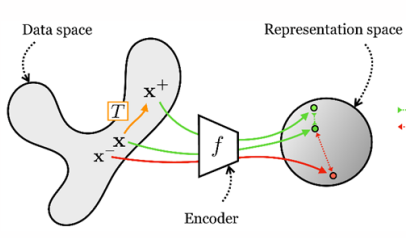
\includegraphics[width=0.6\textwidth]{images/Representation Learning.png}
  \caption{\centering High-level picture of representation learning.
           The encoder $f_\theta$ maps a raw input $\mathbf{x}$ to
           a structured latent vector $\mathbf{z}$, which is then
           used for a downstream task such as classification or
           fairness-aware prediction.}
  \label{fig:repr_learning}
\end{figure}

% , , , , , , , , , , , , , , , , , , , , , , 
\section{Disentangled Representation Learning}
\label{sec:disentangled}
% , , , , , , , , , , , , , , , , , , , , , , 

Standard representation learning makes no assumption about the
\emph{structure} of the latent space.  \emph{Disentangled}
representation learning imposes the additional constraint that
different dimensions (or subspaces) of $\mathbf{z}$ capture
statistically independent generative factors of the data
\cite{bengio2013, higgins2017, kim2018}.

Formally, if the data is generated by $K$ independent factors
$v_1, v_2, \ldots, v_K$, a disentangled encoder should produce
a latent vector $\mathbf{z} = [z_1, z_2, \ldots, z_K]$ such that
\[
  q_\Phi(z_1, z_2, \ldots, z_K)
  \;\approx\;
  \prod_{k=1}^{K} q_\Phi(z_k),
\]
i.e., the joint latent distribution factorises into independent
marginals.  This is precisely the condition that Total Correlation
(Eq.~\ref{eq:total_correlation}) is zero.

\begin{figure}[htbp]
  \centering
  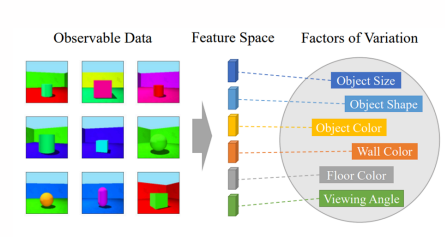
\includegraphics[width=0.8\textwidth]{images/Disentangled.png}
  \caption{Illustration of disentangled representation learning showing mapping from observable data to feature space and factors of variation.}
  \label{fig:disentangled}
\end{figure}
\noindent\textbf{Why does disentanglement matter for fairness?}
If a latent space is properly disentangled, one can isolate and
\emph{remove} the subspace that encodes sensitive demographic
information before passing representations to a downstream
classifier, achieving fairness without sacrificing
task-relevant information.

% , , , , , , , , , , , , , , , , , , , , , , 
\section{Autoencoders}
\label{sec:autoencoders}
% , , , , , , , , , , , , , , , , , , , , , , 

An \emph{autoencoder} is a neural network trained to reconstruct
its input through a bottleneck layer.  It consists of two
components:

\begin{itemize}
  \item \textbf{Encoder} $E_\theta: \mathcal{X} \to \mathcal{Z}$
        compresses the input $\mathbf{x}$ into a latent code
        $\mathbf{z} = E_\theta(\mathbf{x})$.
  \item \textbf{Decoder} $G_\phi: \mathcal{Z} \to \mathcal{X}$
        reconstructs the input as
        $\hat{\mathbf{x}} = G_\phi(\mathbf{z})$.
\end{itemize}

Training minimises reconstruction loss, typically mean-squared error:
\begin{equation}
  \mathcal{L}_{\mathrm{AE}}
  \;=\; \mathbb{E}_{\mathbf{x}}\!\left[
        \bigl\|\mathbf{x} - G_\phi(E_\theta(\mathbf{x}))\bigr\|^2
        \right].
  \label{eq:ae_loss}
\end{equation}
The bottleneck forces the encoder to discard redundant information
and retain only the structure necessary for reconstruction.

\begin{figure}[htbp]
  \centering
  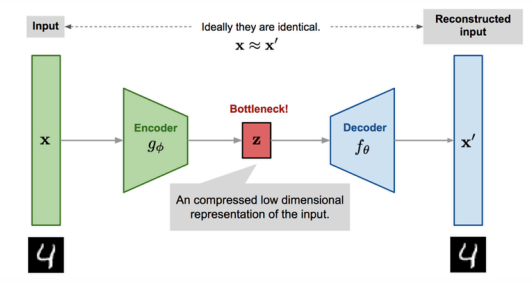
\includegraphics[width=0.8\textwidth]{images/Autoencoder.png}
  \caption{Autoencoder architecture: the encoder $g_\phi$ maps input $\mathbf{x}$ to a low-dimensional latent representation $\mathbf{z}$ (bottleneck), and the decoder $f_\theta$ reconstructs the input as $\mathbf{x'} \approx \mathbf{x}$.}
  \label{fig:autoencoder}
\end{figure}

% , , , , , , , , , , , , , , , , , , , , , , 
\section{Variational Autoencoders (VAE)}
\label{sec:vae}
% , , , , , , , , , , , , , , , , , , , , , , 

A \emph{Variational Autoencoder} (VAE) \cite{kingma2014} is a
probabilistic generative model that frames encoding and decoding
as Bayesian inference.  Instead of mapping an input to a single
point in latent space, the encoder outputs a \emph{distribution}:
\[
  q_\Phi(\mathbf{z}|\mathbf{x})
  = \mathcal{N}\!\bigl(\boldsymbol{\mu}_{q_\Phi}(\mathbf{x}),\;
                        \boldsymbol{\sigma}^2_{q_\Phi}(\mathbf{x})\bigr),
\]
where $\boldsymbol{\mu}$ and $\boldsymbol{\sigma}$ are output by
the encoder network with parameters $\Phi$.  The decoder models
$p_\Theta(\mathbf{x}|\mathbf{z})$.

\noindent\textbf{Reparameterisation trick.}
To enable gradient-based optimisation through a stochastic node,
we sample
\begin{equation}
  \mathbf{z} = \boldsymbol{\mu}_{q_\Phi}(\mathbf{x})
               + \boldsymbol{\sigma}_{q_\Phi}(\mathbf{x}) \odot
               \boldsymbol{\epsilon}, \qquad
  \boldsymbol{\epsilon} \sim \mathcal{N}(\mathbf{0}, \mathbf{I}),
  \label{eq:reparam}
\end{equation}
which moves the randomness outside the computational graph.

\noindent\textbf{Training objective.}
The VAE is trained by maximising the ELBO
(Eq.~\ref{eq:elbo}), which can be written explicitly as:
\begin{equation}
  \mathcal{L}_{\mathrm{VAE}}
  = \sum_{i=1}^{N}
    \Bigl[
      \mathbb{E}_{q_\Phi(\mathbf{z}|\mathbf{x}_i)}\!
      \bigl[\log p_\Theta(\mathbf{x}_i|\mathbf{z})\bigr]
      -
      D_{\mathrm{KL}}\!\bigl(
        q_\Phi(\mathbf{z}|\mathbf{x}_i)\,\|\, p(\mathbf{z})
      \bigr)
    \Bigr].
  \label{eq:vae_loss}
\end{equation}

\noindent\textbf{Extensions for disentanglement.}
$\beta$-VAE \cite{higgins2017} up-weights the KL term by a
hyperparameter $\beta > 1$ to encourage greater disentanglement at
the cost of reconstruction quality.
FactorVAE \cite{kim2018} and $\beta$-TCVAE \cite{chen2018} instead
minimise Total Correlation directly (Eq.~\ref{eq:total_correlation}),
yielding better disentanglement without degrading reconstruction.

% , , , , , , , , , , , , , , , , , , , , , , 
\section{Adversarial Learning}
\label{sec:adversarial}
% , , , , , , , , , , , , , , , , , , , , , , 

\emph{Adversarial learning} is a training paradigm in which two
model components compete in a minimax game, each driving the other
towards a more useful solution \cite{goodfellow2014}.

\subsection{Generative Adversarial Networks (GANs)}

In the canonical GAN setup, a generator $G$ learns to produce
synthetic samples that fool a discriminator $D$, while $D$ learns to
distinguish real from fake:
\begin{equation}
  \min_{G}\;\max_{D}\;
  \mathbb{E}_{\mathbf{x}\sim p_{\mathrm{data}}}\!\bigl[\log D(\mathbf{x})\bigr]
  + \mathbb{E}_{\mathbf{z}\sim p(\mathbf{z})}\!\bigl[\log(1 - D(G(\mathbf{z})))\bigr].
  \label{eq:gan}
\end{equation}
At equilibrium, $G$ produces samples from $p_{\mathrm{data}}$ and $D$
cannot distinguish real from generated samples.

\begin{figure}[htbp]
  \centering
  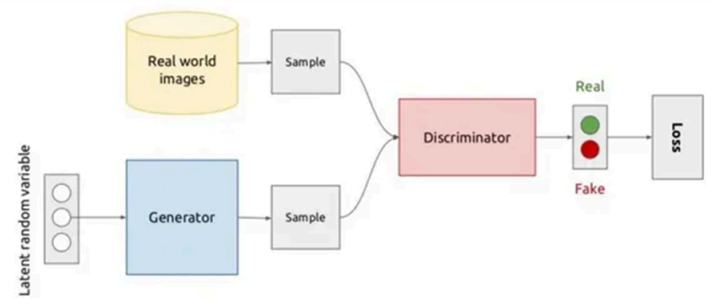
\includegraphics[width=0.85\textwidth]{images/Adversarial .png}
  \caption{Generative Adversarial Network (GAN): the generator maps latent variables to synthetic samples, while the discriminator distinguishes between real and generated data, providing a training signal via adversarial loss.}
  \label{fig:gan}
\end{figure}

\subsection{Adversarial Debiasing}
\label{subsec:adv_debiasing}

In fair representation learning, adversarial networks serve a
different role.  A \emph{predictor} $P$ is trained to predict
a target label $y$ from a representation $\mathbf{z}$, while an
\emph{adversary} $A$ attempts to predict the sensitive attribute
$s$ from the same $\mathbf{z}$.  The encoder is then trained to
\emph{fool the adversary}:
\begin{equation}
  \min_{E,P}\;\max_{A}\;
  \mathcal{L}_{\mathrm{pred}}(P(E(\mathbf{x})),\, y)
  \;-\; \lambda\,\mathcal{L}_{\mathrm{adv}}(A(E(\mathbf{x})),\, s).
  \label{eq:adv_debias}
\end{equation}
The negative sign on the adversarial loss means the encoder
\emph{maximises} the adversary's error—equivalently, it removes
sensitive information from $\mathbf{z}$.

\noindent\textbf{Gradient Reversal Layer (GRL).}
A practical implementation of Eq.~\ref{eq:adv_debias} uses a
Gradient Reversal Layer (GRL) \cite{ganin2016}.  During
the forward pass, GRL acts as the identity; during
back-propagation, it negates the gradient, automatically
implementing the minimax objective without alternating optimisation:
\begin{equation}
  \mathrm{GRL}(\mathbf{z}) = \mathbf{z}, \qquad
  \frac{\partial\,\mathrm{GRL}(\mathbf{z})}{\partial\,\mathbf{z}}
  = -\lambda_{\mathrm{grl}}\,\mathbf{I}.
  \label{eq:grl}
\end{equation}

% , , , , , , , , , , , , , , , , , , , , , , 
\section{Fractional Fourier Transform (FrFT)}
\label{sec:frft}
% , , , , , , , , , , , , , , , , , , , , , , 

The classical Fourier transform maps a signal from the time domain
to the frequency domain.  The \emph{Fractional Fourier Transform}
(FrFT) \cite{ozaktas2001} is a generalisation parameterised by a
rotation order $\alpha \in [0,1]$, interpolating continuously
between the time ($\alpha=0$) and frequency ($\alpha=1$) domains:
\begin{equation}
  \mathcal{F}_\alpha[f](u)
  = \int_{-\infty}^{\infty} f(t)\,K_\alpha(t,u)\,\mathrm{d}t,
  \label{eq:frft}
\end{equation}
where the kernel is
\[
  K_\alpha(t, u)
  = A_\alpha\,
    \exp\!\bigl(
      i\pi(t^2 \cot\alpha - 2tu\csc\alpha + u^2 \cot\alpha)
    \bigr), \qquad
  A_\alpha = \sqrt{1 - i\cot\alpha}.
\]
Deepfake generation pipelines introduce subtle frequency artefacts
that are more discriminative in intermediate spatial–frequency
domains than in either the pure spatial or pure frequency domain
\cite{liu2021}.  By selecting $\alpha$ between 0 and 1, the FrFT
exposes these artefacts while reducing reliance on demographic
appearance features (skin tone, facial structure) that dominate
the spatial domain.

\begin{figure}[htbp]
  \centering
  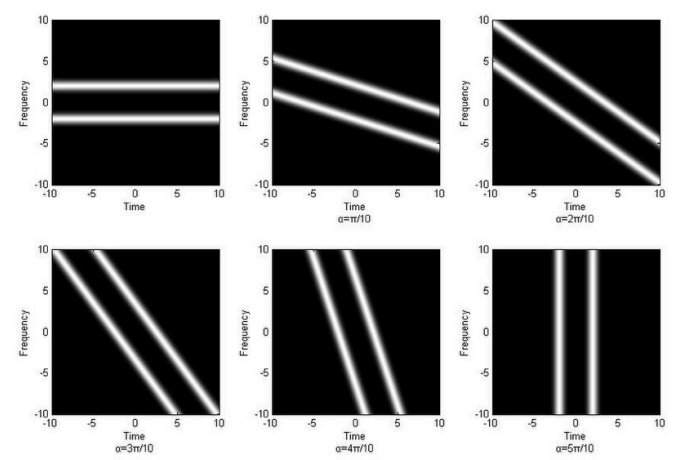
\includegraphics[width=\textwidth]{images/FRFT.png}
  \caption{Fractional Fourier Transform (FRFT) representations at different fractional orders $\alpha$, showing the rotation of signal energy in the time-frequency plane.}
  \label{fig:frft}
\end{figure}

% , , , , , , , , , , , , , , , , , , , , , , 
\section{Fairness Concepts in Machine Learning}
\label{sec:fairness_concepts}
% , , , , , , , , , , , , , , , , , , , , , , 

Before defining evaluation metrics, we establish the terminology
used throughout this report.

\begin{itemize}
  \item \textbf{Target attribute} ($y_t$): the label the model is
        trained to predict (e.g., ``attractive'', ``real/fake'').
  \item \textbf{Protected (sensitive) attribute} ($y_p$):
        a demographic characteristic (e.g., gender, race, age)
        with respect to which the model should \emph{not}
        discriminate.
  \item \textbf{Group fairness}: equal treatment of pre-specified
        demographic groups.
  \item \textbf{Individual fairness}: similar individuals receive
        similar predictions.
\end{itemize}

Let $\hat{Y}$ denote the model's prediction, $Y$ the ground truth
label ($Y=1$ positive, $Y=0$ negative), and $G \in \{g_0, g_1\}$
the protected group membership.  Define:
\begin{align*}
  \mathrm{TPR}_g &= \Pr(\hat{Y}=1 \mid Y=1,\, G=g),
  \quad\text{(True Positive Rate for group }g)\\
  \mathrm{TNR}_g &= \Pr(\hat{Y}=0 \mid Y=0,\, G=g),
  \quad\text{(True Negative Rate for group }g)\\
  \mathrm{FPR}_g &= \Pr(\hat{Y}=1 \mid Y=0,\, G=g).
  \quad\text{(False Positive Rate for group }g)
\end{align*}

% , , , , , , , , , , , , , , , , , , , , , , 
\section{Evaluation Metrics}
\label{sec:eval_metrics}
% , , , , , , , , , , , , , , , , , , , , , , 

\subsection{Equal Opportunity}
\label{subsec:equal_opp}

\emph{Equal Opportunity} \cite{hardt2016} requires that the
True Positive Rate be equal across protected groups.  A model
satisfies equal opportunity if subjects who \emph{deserve} a
positive outcome are equally likely to receive it, regardless
of group membership.  It is measured as:
\begin{equation}
  \Delta_{\mathrm{EO}}
  = \bigl|\mathrm{TPR}_{g_0} - \mathrm{TPR}_{g_1}\bigr|.
  \label{eq:equal_opp}
\end{equation}
A value of $\Delta_{\mathrm{EO}} = 0$ indicates perfect equal
opportunity; \emph{lower is better}.

\subsection{Equalized Odds}
\label{subsec:equalized_odds}

\emph{Equalized Odds} \cite{hardt2016} is a stricter criterion:
the model must achieve equal TPR \emph{and} equal TNR across
groups simultaneously.  This ensures both that qualified
candidates are equally recognised and that unqualified ones are
equally rejected:
\begin{equation}
  \Delta_{\mathrm{EOdd}}
  = \frac{1}{2}\Bigl(
      \bigl|\mathrm{TPR}_{g_0} - \mathrm{TPR}_{g_1}\bigr|
      +
      \bigl|\mathrm{TNR}_{g_0} - \mathrm{TNR}_{g_1}\bigr|
    \Bigr).
  \label{eq:equalized_odds}
\end{equation}
Again, \emph{lower is better}.  The relationship between these
two metrics is: a model satisfying equalized odds also satisfies
equal opportunity, but not vice versa.

\subsection{Standard Accuracy}
\label{subsec:accuracy}

Standard accuracy is the fraction of correctly classified samples:
\begin{equation}
  \mathrm{Acc}
  = \frac{\text{Number of correct predictions}}
         {\text{Total number of predictions}}.
  \label{eq:accuracy}
\end{equation}
While essential for gauging utility, accuracy alone is a misleading
fairness proxy.  On an imbalanced dataset biased towards one
demographic group, a model can achieve high accuracy while
systematically harming an underrepresented group.

\subsection{Equalized Accuracy}
\label{subsec:equalized_acc}

To address the limitations of standard accuracy on skewed test
distributions, the README paper \cite{park2020} introduces
\emph{Equalized Accuracy}, which averages TPR and TNR across
both groups equally:
\begin{equation}
  \mathrm{EAcc}
  = \frac{1}{4}\Bigl(
      \mathrm{TPR}_{g_0} + \mathrm{TNR}_{g_0}
      + \mathrm{TPR}_{g_1} + \mathrm{TNR}_{g_1}
    \Bigr).
  \label{eq:equalized_acc}
\end{equation}
Because each group contributes equally regardless of its size in
the dataset, Equalized Accuracy is a more reliable indicator of
a model's generalisation across the population.

\subsection{FPR-Based Fairness Metrics for Deepfake Detection}
\label{subsec:fpr_metrics}

In the context of deepfake detection, where real faces vastly
outnumber deepfakes in practice, \emph{False Positive Rate}
disparities can have severe societal consequences: real individuals
being misclassified as deepfakes and subjected to unjust scrutiny
\cite{ju2024}.  Three metrics capture this:

\begin{enumerate}
  \item \textbf{FPR Gap} ($G_{\mathrm{FPR}}$): maximum pairwise
        difference in FPR across demographic groups:
        \begin{equation}
          G_{\mathrm{FPR}}
          = \max_{g,g' \in \mathcal{G}}
            \bigl|\mathrm{FPR}_g - \mathrm{FPR}_{g'}\bigr|.
          \label{eq:fpr_gap}
        \end{equation}

  \item \textbf{Equal FPR} ($F_{\mathrm{FPR}}$): summed absolute
        difference between each group's FPR and the overall FPR:
        \begin{equation}
          F_{\mathrm{FPR}}
          = \sum_{g \in \mathcal{G}}
            \left|
              \frac{\sum_i \mathbf{1}[\hat{Y}_i=1,\,G_i=g,\,Y_i=0]}
                   {\sum_i \mathbf{1}[G_i=g,\,Y_i=0]}
              -
              \frac{\sum_i \mathbf{1}[\hat{Y}_i=1,\,Y_i=0]}
                   {\sum_i \mathbf{1}[Y_i=0]}
            \right|.
          \label{eq:equal_fpr}
        \end{equation}

  \item \textbf{Fair Equalized Odds} ($F_{\mathrm{EO}}$):
        extends Equal FPR to both positive and negative classes:
        \begin{equation}
          F_{\mathrm{EO}}
          = \sum_{g \in \mathcal{G}} \sum_{q \in \{0,1\}}
            \left|
              \frac{\sum_i \mathbf{1}[\hat{Y}_i=1,\,G_i=g,\,Y_i=q]}
                   {\sum_i \mathbf{1}[G_i=g,\,Y_i=q]}
              -
              \frac{\sum_i \mathbf{1}[\hat{Y}_i=1,\,Y_i=q]}
                   {\sum_i \mathbf{1}[Y_i=q]}
            \right|.
          \label{eq:fair_eo}
        \end{equation}
\end{enumerate}
For all three metrics, lower values indicate greater fairness.

\subsection{Summary of Metrics}
\label{subsec:metrics_summary}

Table~\ref{tab:metrics_summary} summarises all evaluation metrics,
their target conditions, and the direction of improvement.
\begin{table}[!htbp]
  \centering
  \caption{Summary of fairness and utility evaluation metrics used
           in this report.  All fairness metrics are minimised;
           accuracy metrics are maximised.}
  \label{tab:metrics_summary}
  \small
  \begin{tabular}{llll}
    \toprule
    \textbf{Metric} & \textbf{Symbol} & \textbf{Condition checked}
                    & \textbf{Better} \\
    \midrule
    Equal Opportunity   & $\Delta_{\mathrm{EO}}$     & TPR equal across groups    & $\downarrow$ \\
    Equalized Odds      & $\Delta_{\mathrm{EOdd}}$   & TPR \& TNR equal           & $\downarrow$ \\
    Standard Accuracy   & $\mathrm{Acc}$             & Overall correctness        & $\uparrow$   \\
    Equalized Accuracy  & $\mathrm{EAcc}$            & Balanced group accuracy    & $\uparrow$   \\
    FPR Gap             & $G_{\mathrm{FPR}}$         & Max FPR spread             & $\downarrow$ \\
    Equal FPR           & $F_{\mathrm{FPR}}$         & FPR parity per group       & $\downarrow$ \\
    Fair Equalized Odds & $F_{\mathrm{EO}}$          & TPR \& FPR parity          & $\downarrow$ \\
    AUC-ROC             & AUC                        & Ranking quality            & $\uparrow$   \\
    \bottomrule
  \end{tabular}
\end{table}

% , , , , , , , , , , , , , , , , , , , , , , 
\section{Key Deep Learning Architectures Used in Fair AI}
\label{sec:architectures}
% , , , , , , , , , , , , , , , , , , , , , , 

Table~\ref{tab:model_summary} provides a concise comparison of the
core neural-network models referenced throughout this report.
\begin{table}[!htbp]
  \centering
  \caption{Key model architectures referenced in the fairness-in-AI
           literature covered in this report.}
  \label{tab:model_summary}
  \small
  \begin{tabular}{p{2.4cm}p{3.2cm}p{3.5cm}p{3.5cm}}
    \toprule
    \textbf{Model} & \textbf{Core idea} & \textbf{Strength}
                   & \textbf{Limitation} \\
    \midrule
    VAE \cite{kingma2014}
      & Probabilistic encoder–decoder with Gaussian latent prior
      & Smooth, generative latent space
      & No explicit control over which factors are captured \\
    $\beta$-VAE \cite{higgins2017}
      & Up-weight KL term by $\beta$
      & Encourages disentanglement
      & Hurts reconstruction at high $\beta$ \\
    FactorVAE \cite{kim2018}
      & Minimise Total Correlation via discriminator
      & Better disentanglement than $\beta$-VAE
      & Requires an additional discriminator \\
    FFVAE \cite{creager2019}
      & Disentangle sensitive vs.\ non-sensitive latents
      & Fairness-focused VAE
      & Sensitive latents leak target attribute info \\
    FD-VAE \cite{park2020}
      & Three-way split: TAL, PAL, MAL + decorrelation loss
      & Explicitly decorrelates attributes
      & Requires target \& protected attribute labels \\
    Adversarial Autoencoder
      & GRL to strip demographic info from $\mathbf{z}$
      & Architecture-level fairness
      & Adversarial training instability \\
    FAIR-FRFT (ours)
      & FrFT + adversarial autoencoder + CVaR
      & Frequency-domain fairness
      & Higher computational cost \\
    \bottomrule
  \end{tabular}
\end{table}

% , , , , , , , , , , , , , , , , , , , , , , 
\section{Chapter Summary}
\label{sec:ch2_summary}
% , , , , , , , , , , , , , , , , , , , , , , 

This chapter introduced the mathematical and conceptual vocabulary
needed to follow the technical discussions in subsequent chapters.

\begin{itemize}
  \item \textbf{Mathematical tools}: KL divergence, Total
        Correlation, mutual information, ELBO, and CVaR provide
        the optimisation-theoretic backbone for fair
        representation learning.
  \item \textbf{Architectures}: Autoencoders, VAEs, and adversarial
        networks are the primary building blocks; disentanglement
        methods extend them to produce interpretable, attribute-separable
        latent spaces.
  \item \textbf{FrFT}: Offers a hybrid spatial–frequency domain
        well-suited to capturing deepfake artefacts that are less
        correlated with demographic features.
  \item \textbf{Evaluation metrics}: Equal Opportunity,
        Equalized Odds, Equalized Accuracy, and FPR-based metrics
        together give a multi-dimensional picture of fairness;
        no single metric suffices.
\end{itemize} %background and evaluation metrics
%%  CHAPTER 3
%%  Understanding the README Framework: Representation Learning
%%  by Fairness-Aware Disentangling Method
%%
%%  Based on:  Park et al., arXiv:2007.03775v1 (2020)
%%  Written for the CSC-391 Technical Communication report
%%  "Ethics in AI: Emphasis on Fairness" — Group 7, IITR 2026
%% ============================================================
\setlength{\headheight}{14.5pt}
\addtolength{\topmargin}{-2.5pt}

\chapter{README Framework: Fair Representation Learning Through Disentanglement}
\label{ch:readme}



%% ---- Declaration of Contributions ----------------------------
\vspace{0.5em}
\noindent\rule{\textwidth}{0.4pt}
\textbf{Declaration of Contributions:}
\begin{itemize}[leftmargin=*,noitemsep]
\item \textbf{Pradyuman Singh Shekhawat} — Reviewed key concepts including Variational Autoencoders,
      Total Correlation, and the disentanglement loss derivation; wrote
      Sections~\ref{sec:readme-motivation}--\ref{sec:readme-disentanglement}. Studied and explained the FD-VAE architecture,
      the decorrelation module, and the downstream classification network;
      wrote Sections~\ref{sec:readme-architecture}--\ref{sec:readme-downstream}.
\item \textbf{Vishesh Gupta} — Interpreted the fairness metrics and experimental results;
      wrote Sections~\ref{sec:readme-results}.
\end{itemize}
\noindent\rule{\textwidth}{0.4pt}
\vspace{1em}

% ----------------------------------------------------------------
\section{Motivation and Problem Setting}
\label{sec:readme-motivation}
% ----------------------------------------------------------------

One of the most natural entry-points for tackling bias in machine learning is to attack the problem at
the level of \emph{representation}: if the feature vector that a model learns contains no information
about a sensitive attribute, then any classifier built on top of that vector cannot discriminate on
the basis of that attribute. This idea is the backbone of the \textbf{README} (REpresentation learning
by fairness-Aware Disentangling MEthod) paper by Park \emph{et al.}~\cite{park2020readme}.

Formally, let us denote the observed data by $\mathcal{X} = \{x_1, \ldots, x_n\}$, the target
attribute labels by $\mathcal{Y}_t = \{y_{t_1}, \ldots, y_{t_n}\}$, and the protected attribute
labels by $\mathcal{Y}_p = \{y_{p_1}, \ldots, y_{p_n}\}$. A protected attribute is any characteristic
such as \emph{gender}, \emph{age}, or \emph{race} on which individuals ought not to be
discriminated against. A target attribute is the quantity the downstream classifier is actually
supposed to predict, e.g., whether a face is \emph{attractive} or whether the hair is
\emph{wavy}. The challenge is that in real-world datasets, target and protected attributes are
often statistically correlated --- for example, the ``attractive'' label in the CelebA dataset is
influenced by the gender distribution in the data~\cite{park2020readme}.

\subsection{Limitation of Earlier Disentanglement Approaches}
\label{ssec:readme-ffvae-limitation}

Prior to README, the state-of-the-art approach for fair representation learning via disentanglement was
\textbf{FFVAE} (Flexibly Fair Variational AutoEncoder) by Creager~\emph{et al.}~\cite{creager2019ffvae}.
FFVAE partitions the latent space into two parts:
\begin{itemize}
    \item \emph{Sensitive latents}: latent variables trained to be highly informative about the
          protected attribute; and
    \item \emph{Non-sensitive latents}: latent variables trained to be independent of the sensitive
          latents.
\end{itemize}
During downstream classification, only the non-sensitive latents are used, with the reasoning that
this excludes all protected-attribute information from the prediction pipeline.

Park~\emph{et al.} identify a fundamental flaw in this two-way split. Because real-world attributes
are correlated, the sensitive latents end up capturing \emph{both} protected-attribute information
\emph{and} some target-attribute information. When these latents are excluded for fairness, useful
discriminative signal for the target task is discarded along with the demographic information. The
authors demonstrate this empirically: when they perform downstream classification using each
subspace independently on the CelebA dataset (target attribute = \emph{attractive}, protected
attribute = \emph{male}), the sensitive latents actually produce \emph{higher} accuracy on the
target attribute than the non-sensitive latents (67.4\% vs 62.7\%), revealing that excluding them
comes at an unnecessary accuracy cost.

This observation motivates the central design choice of README: the latent space should be split into
\emph{three} independent subspaces, not two --- separating target information, protected information,
and the \emph{shared} information predictive of both into its own dedicated slot.

\begin{figure}[htbp]
    \centering
    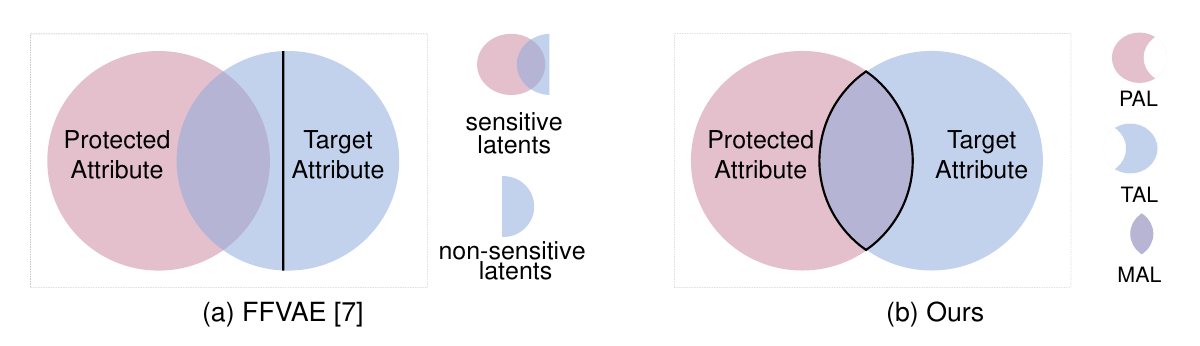
\includegraphics[width=\textwidth]{figures/readme-motivation.png}
    \caption{
        Motivation for fairness-aware disentanglement.
        (a) Prior methods (e.g., FFVAE) mix target and protected information, causing loss of useful features.
        (b) README separates them into TAL, PAL, and MAL, isolating shared information without harming performance.
    }
    \label{fig:readme-motivation}
\end{figure}
% ----------------------------------------------------------------
\section{Overview of the FD-VAE Architecture}
\label{sec:readme-architecture}
% ----------------------------------------------------------------

The README framework is built around a model called the \textbf{Fairness-aware Disentangling
Variational AutoEncoder (FD-VAE)}. At a high level, the FD-VAE is a VAE extended with two additional
components: a discriminator for encouraging disentanglement across the three subspaces, and a
decorrelation module that explicitly specifies \emph{which type} of information should reside in
each subspace.

The architecture operates in two stages:
\begin{enumerate}
    \item \textbf{Representation Learning Stage}: The FD-VAE (encoder + decoder + discriminator +
          decorrelation module) is trained jointly to produce a well-disentangled and decorrelated
          latent space.
    \item \textbf{Downstream Classification Stage}: The encoder is frozen, and a lightweight
          classification network is trained on the learned latent variables to predict the target
          attribute in a fairness-preserving manner.
\end{enumerate}

\begin{figure}[htbp]
    \centering
    % Replace the placeholder with the actual architecture figure from the paper
    % or the one recreated in Chapter figures/fdvae_architecture.pdf
    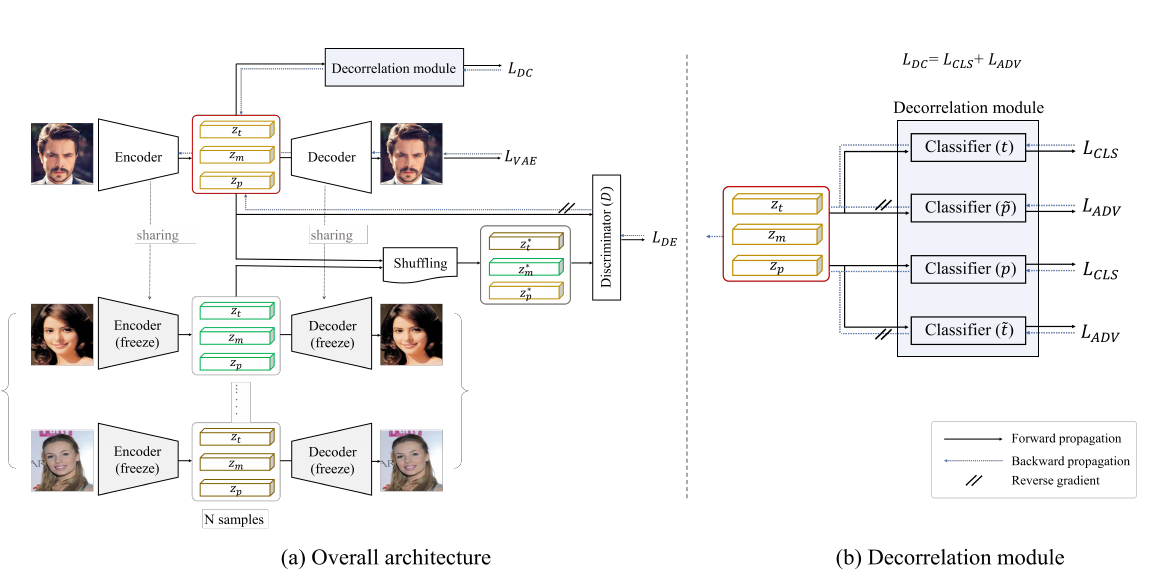
\includegraphics[width=\linewidth]{figures/readme-architecture.png}
    \caption{%
        Full architecture of the Fairness-aware Disentangling VAE (FD-VAE).
        Source: adapted from Park \emph{et al.}~\cite{park2020readme}.
    }
    \label{fig:fdvae-overview}
\end{figure}

\subsection{The Three Latent Subspaces}

The encoder $q_\Phi(z \mid x)$ maps an input image to three independent latent subspaces:

\begin{description}
    \item[Target Attribute Latent (TAL), $z_t$.]  This subspace is trained to carry only the
          information that is predictive of the target attribute $y_t$. During representation learning
          it receives a supervised classification signal for $y_t$ and an adversarial signal that
          prevents it from leaking protected-attribute information.

    \item[Protected Attribute Latent (PAL), $z_p$.]  Symmetrically, this subspace is trained to
          contain only protected-attribute information $y_p$. Because it carries the demographic
          signal, it is \emph{excluded entirely} from the downstream classification pipeline to ensure
          that the final predictor cannot use demographic information.

    \item[Mutual Attribute Latent (MAL), $z_m$.]  This is the key novelty of README. In real datasets
          there exists information that is predictive of \emph{both} $y_t$ and $y_p$ simultaneously
          (e.g., facial structure features that correlate with both attractiveness and gender). If this
          shared information were forced into either TAL or PAL, it would violate the decorrelation
          objective. MAL provides a dedicated ``overflow'' subspace for this information. During
          downstream classification, the protected-attribute signal in MAL is stripped away before
          MAL's remaining content is used to augment the classification.
\end{description}

In all experiments, each subspace is set to 20 dimensions, for a total latent dimension of 60.

% ----------------------------------------------------------------
\section{The Variational Autoencoder Objective}
\label{sec:readme-vae}
% ----------------------------------------------------------------

The encoder and decoder follow the standard VAE formulation of Kingma and
Welling~\cite{kingma2014vae}. The encoder outputs mean and variance parameters
$(\mu, \sigma) = q_\Phi(x)$, from which latent codes are drawn via the reparameterisation trick:
\[
    z \sim \mathcal{N}\!\left(\mu_{q_\Phi}(x),\, \sigma_{q_\Phi}(x)\right).
\]
The VAE objective is to maximise the Evidence Lower Bound (ELBO):
\begin{equation}
    L_\text{VAE} = \sum_{i=1}^{n}
        \mathbb{E}_{q_\Phi(z_t, z_p, z_m \mid x_i)}\!\left[
            \log p_\Theta(x_i \mid z_t, z_p, z_m)
        \right]
        - \mathrm{KL}\!\left[
            q_\Phi(z_t, z_p, z_m \mid x_i)
            \,\|\,
            p(z_t, z_p, z_m)
        \right].
    \label{eq:vae-elbo}
\end{equation}
The first term is the \emph{reconstruction loss}: the decoder $p_\Theta$ tries to faithfully
reconstruct each input from the concatenated latent codes $(z_t, z_p, z_m)$. The second term
is the \emph{KL regularisation loss}: it encourages the posterior $q_\Phi$ to remain close to
the standard Gaussian prior $p(z) = \mathcal{N}(0, I)$, which acts as a regulariser and ensures
the latent space has good coverage.

% ----------------------------------------------------------------
\section{Disentanglement Loss via Total Correlation}
\label{sec:readme-disentanglement}
% ----------------------------------------------------------------

The VAE objective alone does not enforce that the three subspaces $z_t$, $z_p$, and $z_m$ are
\emph{mutually independent}. Mutual independence between subspaces is formalised using the
\textbf{Total Correlation (TC)}~\cite{watanabe1960tc}, which is the KL divergence between the joint
distribution and the product of its marginals:
\begin{equation}
    L_\text{DE} = \mathrm{KL}\!\left[
        q_\Phi(z_t, z_p, z_m)
        \,\Big\|\,
        \prod_{j \in S} q_\Phi(z_j)
    \right]
    = \mathbb{E}_{q_\Phi(z_t, z_p, z_m)}\!\left[
        \log \frac{q_\Phi(z_t, z_p, z_m)}{\prod_{j \in S} q_\Phi(z_j)}
    \right],
    \label{eq:tc}
\end{equation}
where $S = \{t, p, m\}$. Minimising the Total Correlation forces the three subspaces to become
maximally independent of each other, which is the formal definition of disentanglement.

\subsection{Adversarial Approximation of the Discriminator}

Directly computing the log-density ratio in Equation~\eqref{eq:tc} is intractable. Following the
approach of Kim and Mnih~\cite{kim2018factorVAE}, the log-density ratio is approximated by training
a discriminator $D$ to classify between \emph{real samples} (drawn from the joint $q_\Phi(z_t, z_p, z_m)$)
and \emph{fake samples} $z^* = [z_t^*; z_p^*; z_m^*]$ generated by independently shuffling each
subspace within a mini-batch:
\begin{equation}
    L_\text{DE} \approx \mathbb{E}_{q_\Phi(z_t, z_p, z_m)}\!\left[
        \log \frac{D(z_t, z_p, z_m)}{1 - D(z_t, z_p, z_m)}
    \right].
    \label{eq:tc-approx}
\end{equation}
The discriminator is trained separately to classify real vs.\ fake by minimising:
\begin{equation}
    L_D = -\mathbb{E}_{q_\Phi(z_t, z_p, z_m)}\!\left[
        \log D(z_t, z_p, z_m) + \log\!\left(1 - D(z_t^*, z_p^*, z_m^*)\right)
    \right].
    \label{eq:disc-loss}
\end{equation}
The encoder $q_\Phi$ is simultaneously trained to fool the discriminator, which drives the Total
Correlation toward zero and therefore encourages independence between the three subspaces.

% ----------------------------------------------------------------
\section{Decorrelation Loss}
\label{sec:readme-decorrelation}
% ----------------------------------------------------------------

The disentanglement loss ensures that the three subspaces are \emph{statistically independent}, but
it says nothing about \emph{which information goes where}. The decorrelation loss $L_\text{DC}$
takes over this role: it provides explicit supervision to ensure that $z_t$ contains target
attribute information, $z_p$ contains protected attribute information, and each is purged of the
other's signal.

The decorrelation loss is composed of two terms:
\begin{equation}
    L_\text{DC} = \beta L_\text{CLS} + \gamma L_\text{ADV},
    \label{eq:dc}
\end{equation}
where $\beta$ and $\gamma$ are hyperparameters (set to 5 and 10, respectively, in all experiments).

\subsection{Classification Loss \texorpdfstring{$L_\text{CLS}$}{L\_CLS}}
\label{ssec:lcls}

The classification loss provides direct supervision to assign the correct information to the correct
subspace. It minimises cross-entropy for predicting the target label $y_t$ from $z_t$, and for
predicting the protected label $y_p$ from $z_p$:
\begin{equation}
    L_\text{CLS} = -\sum_{i=1}^{n}
        \mathbb{E}_{q_\Phi(z_t, z_p, z_m \mid x_i)}\!\Big[
            \log p_t(y_{t_i} \mid z_t) + \log p_p(y_{p_i} \mid z_p)
        \Big],
    \label{eq:lcls}
\end{equation}
where $p_t$ and $p_p$ are lightweight classifiers (single fully-connected layers) trained to predict the
target and protected attributes from their respective subspaces.

\subsection{Adversarial Loss \texorpdfstring{$L_\text{ADV}$}{L\_ADV}}
\label{ssec:ladv}

The classification loss alone is not enough: it pushes the correct information \emph{into} each
subspace but does not actively remove unwanted cross-information. The adversarial loss does this by
training two adversarial classifiers $\tilde{p}$ (predicting $y_p$ from $z_t$) and $\tilde{t}$
(predicting $y_t$ from $z_p$), and using \emph{reverse gradients} to force the encoder to make these
classifiers fail:
\begin{equation}
    L_\text{ADV} = \max_{\tilde{t},\, \tilde{p}}\;
        \min_{\Phi}\; \sum_{i=1}^{n}
        \mathbb{E}_{q_\Phi(z_t, z_p, z_m \mid x_i)}\!\Big[
            \log p_{\tilde{p}}(y_{p_i} \mid z_t) + \log p_{\tilde{t}}(y_{t_i} \mid z_p)
        \Big].
    \label{eq:ladv}
\end{equation}
The minimax structure is crucial: the adversarial classifiers $\tilde{p}$ and $\tilde{t}$ are
trained to \emph{maximise} their ability to predict cross-attribute labels, while the encoder
$q_\Phi$ is trained to \emph{minimise} this ability. This creates a game that drives protected-attribute
information out of $z_t$ and target-attribute information out of $z_p$.

\subsection{The Role of the Mutual Attribute Latent in Decorrelation}

A key subtlety is what happens to information that is genuinely predictive of \emph{both} attributes
simultaneously. Forcing this information into either $z_t$ or $z_p$ would increase $L_\text{ADV}$ in
either direction. The MAL $z_m$ acts as a pressure valve: the disentanglement loss $L_\text{DE}$
indirectly encourages this shared information to migrate into $z_m$, because placing it there
satisfies both the independence constraint and keeps $L_\text{ADV}$ low. No additional explicit
mapping is applied to $z_m$ during representation learning.

\subsection{Total Objective for Stage 1}

The full representation learning objective that the FD-VAE maximises is:
\begin{equation}
    L_\text{TOTAL} = L_\text{VAE} - \alpha L_\text{DE} - L_D - L_\text{DC},
    \label{eq:total}
\end{equation}
where $\alpha$ is a hyperparameter controlling the strength of the disentanglement
objective ($\alpha = 50$ in all experiments). The negative signs on $L_\text{DE}$ and $L_D$ reflect
the fact that the encoder is trained to \emph{minimise} Total Correlation (thus maximise the negated
discriminator objective), while the discriminator $D$ is trained separately to minimise $L_D$.

% ----------------------------------------------------------------
\section{Downstream Classification Network}
\label{sec:readme-downstream}
% ----------------------------------------------------------------

Once Stage 1 training is complete, the encoder weights are frozen and the downstream classification
network is trained to predict $y_t$ in a fair manner.

\paragraph{Excluding PAL.}
The Protected Attribute Latent $\hat{z}_p$ is dropped entirely. Because the decorrelation objective
has already separated all target-attribute information out of $\hat{z}_p$, this exclusion does not
hurt target-prediction accuracy while guaranteeing that the final classifier has no access to
demographic information.

\paragraph{Sanitising MAL.}
The Mutual Attribute Latent $\hat{z}_m$ still carries some residual protected-attribute signal (since
it holds the shared information). A single fully connected layer $f$ is applied to $\hat{z}_m$ to
produce a transformed representation $z_n$. An adversarial protected-attribute classifier $\tilde{d}$
is trained to extract demographic information from $z_n$ via reverse gradients, and $f$ is trained
to defeat $\tilde{d}$:
\begin{align}
    L_\text{DCLS} &= \max_{d,\, f}\; \min_{\tilde{d}}\; \sum_{i=1}^{n}
        \mathbb{E}_{q_\Phi(\hat{z}_t, \hat{z}_p, \hat{z}_m \mid x_i)}\!\Big[
            \log p_d\!\left(y_{t_i} \mid \hat{z}_t \oplus f(\hat{z}_m)\right)
            - \log p_{\tilde{d}}\!\left(y_{p_i} \mid f(\hat{z}_m)\right)
        \Big],
    \label{eq:dcls}
\end{align}
where $\oplus$ denotes element-wise summation and $d$ is the final target-attribute classifier.

\paragraph{Combining TAL and sanitised MAL.}
The sanitised representation $z_n$ (from $f(\hat{z}_m)$) is added element-wise to $\hat{z}_t$ and
the result is fed into the classifier $d$. This combination leverages the rich shared information
captured in MAL (now stripped of its demographic component) to boost the discriminative power of the
final prediction beyond what $\hat{z}_t$ alone could achieve.

Figure~\ref{fig:downstream} illustrates the downstream classification architecture.

\begin{figure}[htbp]
    \centering
    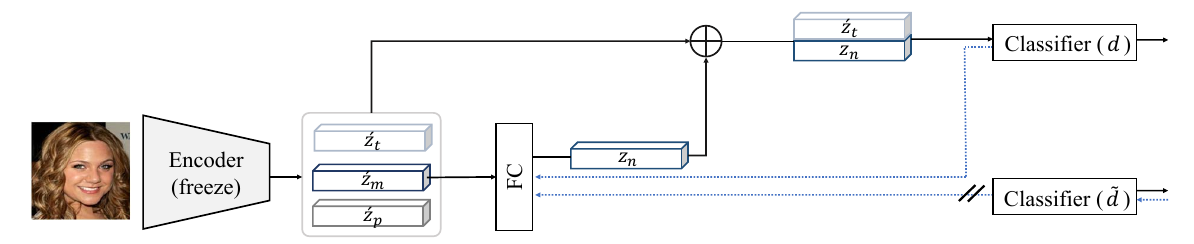
\includegraphics[width=0.75\linewidth]{figures/readme-downstream.png}
    \caption{%
        Downstream classification network of FD-VAE. Source: adapted from Park~\emph{et al.}~\cite{park2020readme}.
    }
    \label{fig:downstream}
\end{figure}

% ----------------------------------------------------------------
\section{Datasets}
\label{sec:readme-datasets}
% ----------------------------------------------------------------

\paragraph{CelebA.}
The CelebA dataset~\cite{liu2015celeba} consists of approximately 200\,000 celebrity face images,
each annotated with 40 binary attributes. The authors consider four (protected, target) attribute
pairs drawn from the attributes \textit{male} (M), \textit{young} (Y), \textit{attractive} (A),
\textit{wavy hair} (W), and \textit{big nose} (B):
\[
    (\text{M},\,\text{A}), \quad (\text{M},\,\text{W}), \quad (\text{Y},\,\text{A}), \quad (\text{Y},\,\text{B}).
\]

\paragraph{UTK Face.}
The UTK Face dataset~\cite{zhang2017utkface} contains face images spanning a wide age range,
annotated for age, ethnicity, and gender. Gender is used as the protected attribute, while ethnicity
(binarised into Caucasian vs.\ others) and age (binarised into young vs.\ older than 35) serve as
target attributes. The training split is constructed to be \emph{imbalanced} between the protected
and target attributes, creating a realistic fairness challenge; the validation and test sets are
balanced.

% ----------------------------------------------------------------
\section{Experimental Results}
\label{sec:readme-results}
% ----------------------------------------------------------------

Table~\ref{tab:celeba-results} and Table~\ref{tab:utk-results} present the classification results on
CelebA and UTK Face datasets, respectively, comparing FD-VAE against four baselines: a plain VAE
(no fairness consideration), $\beta$-VAE, FactorVAE, and FFVAE. For each dataset the baseline
methods are evaluated with the same 60-dimensional representation to ensure a fair comparison.

\subsection{Results on CelebA}

\begin{table}[htbp]
    \centering
    \caption{%
        Classification results on the CelebA dataset. M = male, Y = young, A = attractive,
        W = wavy hair, B = big nose. PA = protected attribute, TA = target attribute.
        $\downarrow$ indicates lower is better (fairer); $\uparrow$ indicates higher is better.
        Bold entries indicate the best result in each column. Source: Park~\emph{et al.}~\cite{park2020readme}.
    }
    \label{tab:celeba-results}
    \small
    \setlength{\tabcolsep}{5pt}
    \begin{tabular}{lllcccc}
        \toprule
        \textbf{Method} & \textbf{TA} & \textbf{PA} &
        \textbf{Equal Opp.~$\downarrow$} & \textbf{Eq.\ Odds~$\downarrow$} &
        \textbf{Acc.~$\uparrow$} & \textbf{Eq.\ Acc.~$\uparrow$} \\
        \midrule
        VAE             & A & M & 27.2 & 28.7 & 70.6 / 65.3 & --- \\
        $\beta$-VAE     & A & M & 21.1 & 22.1 & 68.7 / 64.6 & --- \\
        FactorVAE       & A & M & 20.7 & 23.4 & 69.0 / 64.9 & --- \\
        FFVAE           & A & M & 17.7 & 17.5 & 62.7 / 59.5 & --- \\
        \textbf{FD-VAE (Ours)} & A & M & \textbf{1.3} & \textbf{4.9} & 64.1 / 63.5 & --- \\
        \midrule
        VAE             & W & M & 47.1 & 33.4 & 73.0 / 59.0 & --- \\
        $\beta$-VAE     & W & M & 35.4 & 15.3 & 70.7 / 57.3 & --- \\
        FactorVAE       & W & M & 38.8 & 28.8 & 71.0 / 58.0 & --- \\
        FFVAE           & W & M & 21.1 & 15.4 & 67.7 / 54.3 & --- \\
        \textbf{FD-VAE (Ours)} & W & M & \textbf{13.4} & \textbf{8.9}  & 66.1 / 52.9 & --- \\
        \midrule
        VAE             & A & Y &  9.7 & 11.3 & 70.9 / 69.6 & --- \\
        FFVAE           & A & Y &  8.0 &  8.2 & 64.2 / 62.9 & --- \\
        \textbf{FD-VAE (Ours)} & A & Y & \textbf{3.7} & \textbf{1.9} & 65.5 / 66.0 & --- \\
        \midrule
        VAE             & B & Y & 17.0 & 19.2 & 67.2 / 64.0 & --- \\
        FFVAE           & B & Y &  5.3 &  8.5 & 63.0 / 58.2 & --- \\
        \textbf{FD-VAE (Ours)} & B & Y & \textbf{1.2} & \textbf{1.5} & 63.9 / 57.7 & --- \\
        \bottomrule
    \end{tabular}
\end{table}

The results are striking. On the (M, A) pair, FD-VAE reduces the equal opportunity gap from
FFVAE's 17.7\% to just \textbf{1.3\%} --- a reduction of 16.4 percentage points. Similarly, the
equalized-odds gap falls from 17.5\% to \textbf{4.9\%}. Across all four attribute pairs on CelebA,
FD-VAE consistently outperforms FFVAE by large margins on both fairness metrics while maintaining
comparable accuracy (within 1--2\% of FFVAE on equalized accuracy). This confirms that the
three-way disentanglement preserves more discriminative signal for the target task than the simpler
two-way split of FFVAE.

\subsection{Results on UTK Face}

\begin{table}[htbp]
    \centering
    \caption{%
        Classification results on the UTK Face dataset. G = gender (protected),
        E = ethnicity (target), A = age (target).
        $\downarrow$ = lower is better; $\uparrow$ = higher is better.
        Bold = best result. Source: Park~\emph{et al.}~\cite{park2020readme}.
    }
    \label{tab:utk-results}
    \small
    \setlength{\tabcolsep}{5pt}
    \begin{tabular}{lllcccc}
        \toprule
        \textbf{Method} & \textbf{TA} & \textbf{PA} &
        \textbf{Equal Opp.~$\downarrow$} & \textbf{Eq.\ Odds~$\downarrow$} &
        \textbf{Acc.~$\uparrow$} \\
        \midrule
        VAE         & E & G & 16.1 & 17.4 & 65.2 \\
        $\beta$-VAE & E & G & 12.7 & 12.1 & 60.1 \\
        FactorVAE   & E & G & 12.1 & 12.9 & 59.4 \\
        FFVAE       & E & G &  9.8 &  9.1 & 59.7 \\
        \textbf{FD-VAE} & E & G & \textbf{2.3} & \textbf{1.1} & 60.3 \\
        \midrule
        VAE         & A & G & 24.6 & 29.8 & 60.7 \\
        $\beta$-VAE & A & G & 17.1 & 20.8 & 54.3 \\
        FactorVAE   & A & G & 23.2 & 27.1 & 54.6 \\
        FFVAE       & A & G & 13.6 & 17.2 & 54.5 \\
        \textbf{FD-VAE} & A & G & \textbf{2.0} & \textbf{2.9} & 54.1 \\
        \bottomrule
    \end{tabular}
\end{table}

On UTK Face, FD-VAE achieves 2.3\% and 2.0\% equal opportunity for the ethnicity and age
classification tasks respectively --- reductions of roughly 7 to 11 percentage points over FFVAE
with no meaningful drop in accuracy. This demonstrates that the improvement generalises across
different datasets and protected-attribute types.

% ----------------------------------------------------------------
\section{Summary}
\label{sec:readme-summary}
% ----------------------------------------------------------------

The README framework makes three distinct contributions to fair representation learning, which we
briefly recap here before connecting them to the broader context of the report:

\begin{description}
    \item[Three-way latent disentanglement.] By introducing the Mutual Attribute Latent as a
          third subspace alongside the target and protected attribute latents, README avoids the
          information leak that afflicts two-way disentanglement approaches. This single design
          change enables a far cleaner separation of attribute-specific information.

    \item[Explicit decorrelation via adversarial supervision.] The decorrelation loss goes beyond
          generic disentanglement: it provides direct supervision via $L_\text{CLS}$ to assign
          correct information to each subspace, and adversarially removes unwanted cross-information
          via $L_\text{ADV}$. This two-pronged approach is shown in the ablation study to be the
          decisive factor for fairness.

    \item[Novel equalized accuracy metric.] By proposing an accuracy metric that weights all
          group--outcome combinations equally, README provides the community with a tool that is
          immune to dataset imbalance, making comparisons across skewed benchmarks more meaningful.
\end{description}

The experimental results on CelebA and UTK Face demonstrate that FD-VAE outperforms all prior
methods by substantial margins on standard fairness metrics (equal opportunity, equalized odds),
while achieving comparable accuracy. The framework lays the groundwork for the application we
explore in Chapter~\ref{ch:cvar_deepfake}: extending fairness-aware representation learning to the
more challenging problem of deepfake detection.

\vspace{2em}
% ---- Chapter Bibliography Note --------------------------------
\noindent\textit{The primary reference for this chapter is Park~\emph{et al.}, ``README: REpresentation
learning by fairness-Aware Disentangling MEthod,'' arXiv:2007.03775v1, 2020. All tables and figures
are adapted from this paper.} %readME
%% ============================================================
%% CHAPTER 4 — CVaR-Based Fair Deepfake Detection: DAG-FDD and DAW-FDD
%% ============================================================

\chapter{CVaR-Based Fair Deepfake Detection: DAG-FDD and DAW-FDD}
\label{ch:cvar_deepfake}



\vspace{0.5em}
\noindent\rule{\textwidth}{0.4pt}
\textbf{Declaration of Contributions:} This chapter was primarily authored by \textit{Aryan Choudhary}, who conducted a detailed study of the referenced work, systematically extracted its mathematical formulations and reformulated the methodology into this report chapter. The presentation of CVaR-based robust optimization along with demographic-agnostic and demographic-aware fairness frameworks was carefully structured and formalized to align with the objectives of the literature review. All mathematical expressions and derivations were rigorously verified to ensure consistency with the original paper.
\noindent\rule{\textwidth}{0.4pt}
\vspace{1em}

\bigskip
% ------------------------------------------------------------------ 
\section{Introduction}
\label{sec:ch4_intro}
% ------------------------------------------------------------------

In this chapter, we review the fairness oriented deepfake detection framework proposed in \cite{dag_paper}, with particular emphasis on the role of Conditional Value-at-Risk (CVaR) in robust optimisation. The central idea is that conventional training, which minimises average loss, tends to prioritise easy and dominant samples. In deepfake detection, this can lead to uneven performance across hidden or explicit demographic groups: a model may achieve strong overall accuracy while still producing substantially higher error rates for certain subpopulations.

To address this limitation, the paper introduces two related training strategies:

\begin{itemize}
    \item \textbf{DAG-FDD} (Demographic-Agnostic Fair Deepfake Detection) : used when demographic labels are \emph{not} available.
    \item \textbf{DAW-FDD} (Demographic-Aware Fair Deepfake Detection) : used when demographic labels \emph{are} available.
\end{itemize}

Both methods are built on the same broad principle: instead of optimising the average loss over all samples, the training procedure is modified to emphasise the worst-performing samples or groups. This makes the detector more robust and in the fairness setting, reduces the likelihood that the model performs well only on majority or easy cases. 

The contribution of this paper \cite{dag_paper} is particularly significant as it demonstrates that fairness can be incorporated through the objective function without requiring changes to the underlying detection architecture. Since the fairness behavior is largely governed by the loss formulation, the approach remains flexible and can be extended to a wide range of models.


% ------------------------------------------------------------------
\section{Background: Why Average Loss Is Not Enough}
\label{sec:ch4_avg_loss}
% ------------------------------------------------------------------

Standard learning methods minimise the expected loss

\begin{equation}
    R_{\mathrm{avg}}(\theta)
    = \mathbb{E}_{(X,Y)\sim P}\bigl[\ell(\theta;\,X,Y)\bigr],
    \label{eq:avg_risk}
\end{equation}

\noindent where $\theta$ denotes the model parameters, $(X,Y)$ is a training sample drawn from data distribution $P$, and $\ell(\theta;X,Y)$ is the prediction loss. This objective treats every sample equally on average. While effective for ordinary accuracy maximisation, it is not suitable when the dataset contains imbalance across subgroups: a model can reduce its total average loss by doing well on dominant or easier samples, even if it performs poorly on minority or difficult groups.

This is exactly the limitation which we try to overcome. The authors of \cite{dag_paper} argue that fairness in deepfake detection should not be measured only through average behaviour, because the average can hide worst-case performance. A detector that fails badly on one group but performs well on others may still appear strong under standard metrics. Therefore, the paper replaces average-risk training with a \emph{robust risk} objective.

% ------------------------------------------------------------------
\section{CVaR as the Core Robustness Principle}
\label{sec:cvar_core}
% ------------------------------------------------------------------

The paper \cite{dag_paper} uses \textbf{Conditional Value-at-Risk (CVaR)} as the main robust optimisation tool. CVaR is a classical idea from risk-sensitive optimisation; it focuses on the \emph{tail} of the loss distribution rather than its mean. For a given parameter vector $\theta$, the CVaR objective is

\begin{equation}
    \mathrm{CVaR}_{\alpha}(\theta)
    = \inf_{\lambda \in \mathbb{R}}
      \left\{
        \lambda
        + \frac{1}{\alpha}\,
          \mathbb{E}_{(X,Y)\sim P}
          \bigl[\,[\ell(\theta;\,X,Y) - \lambda]_{+}\,\bigr]
      \right\}
    \label{eq:cvar}
\end{equation}

\textit{The notion of infimum has been formally introduced in Chapter~\ref{ch:background}.}


\noindent where $[a]_{+} = \max(0,\,a)$.

\subsection{Interpretation of the variables}
\label{subsec:cvar_vars}

Here, $\lambda$ is a threshold or pivot value. The expression $[\ell(\theta;X,Y)-\lambda]_{+}$ retains only the part of the loss that exceeds $\lambda$: samples whose losses are below the threshold contribute nothing, while samples above the threshold contribute proportionally to how badly the model performs on them.

The parameter $\alpha \in (0,1)$ determines the fraction of the highest-loss region that is emphasised. A smaller $\alpha$ concentrates more strongly on the hardest samples, while a larger $\alpha$ makes the objective closer to average loss. This makes $\alpha$ an important hyperparameter in controlling how \emph{aggressively} the model focuses on the difficult portion of the data.

\subsection{Intuition}
\label{subsec:cvar_intuition}

The intuition behind CVaR is simple but powerful: instead of asking ``How well does the model perform on average?'', it asks ``How bad is the model on the worst fraction of cases?'' This is especially useful in fairness-sensitive applications, because the worst fraction of cases is often where minority or underrepresented groups appear.

% ------------------------------------------------------------------
\section{DAG-FDD: Demographic-Agnostic Fair Deepfake Detection}
\label{sec:dag_fdd}
% ------------------------------------------------------------------

\subsection{Motivation}
\label{subsec:dag_motivation}

DAG-FDD is used when demographic labels are not available which is a realistic scenario in many deepfake detection settings, since training sets may not contain explicit annotations for race, sex, age or other sensitive attributes. Even without demographic labels, the data may still contain \emph{latent groups}, some of which may be harder to classify than others. DAG-FDD is designed to reduce the risk that the detector performs disproportionately poorly on such hidden subgroups.

\subsection{Latent-Group Formulation}
\label{subsec:dag_latent}

The paper models the overall data distribution as a mixture of $K$ latent group distributions:

\begin{equation}
    P = \sum_{m=1}^{K} \pi_m\, P_m
    \label{eq:mixture}
\end{equation}

\noindent where $P_m$ is the distribution of the $m$-th latent group, $\pi_m$ is its mixture weight, and $\sum_m \pi_m = 1$. The corresponding worst-group risk is

\begin{equation}
    R_{\max}(\theta)
    = \max_{m=1,\ldots,K}\;
      \mathbb{E}_{(X,Y)\sim P_m}\bigl[\ell(\theta;\,X,Y)\bigr]
    \label{eq:worst_group_risk}
\end{equation}

This objective directly represents the fairness concern: instead of minimising the mean risk across all groups, we control the risk of the worst group.

\subsection{Why CVaR Helps in the Demographic-Agnostic Setting}
\label{subsec:dag_cvar_bound}

The paper \cite{dag_paper} shows that CVaR on sample losses can act as an upper-bound surrogate for worst-group risk when $\alpha$ is small enough. Specifically, if

\begin{equation}
    \alpha \;\leq\; \min_{m}\;\pi_m
    \label{eq:alpha_bound}
\end{equation}

\noindent then the CVaR objective provides an upper bound on the maximum group risk. This result is important because it justifies using sample-level CVaR even when group labels are missing. The practical meaning is that the hardest samples in the overall dataset tend to come from the hardest latent groups; therefore, if training is forced to pay greater attention to the worst samples, the model indirectly becomes more robust to hidden demographic imbalance.

\subsection{Empirical Objective Used in DAG-FDD}
\label{subsec:dag_objective}

For a dataset of size $n$, the empirical DAG-FDD objective is

\begin{equation}
    \mathcal{L}_{\mathrm{DAG\text{-}FDD}}(\theta,\lambda)
    = \lambda
      + \frac{1}{\alpha n}
        \sum_{i=1}^{n}
        \bigl[\ell(\theta;\,X_i,Y_i) - \lambda\bigr]_{+}
    \label{eq:dag_obj}
\end{equation}

\noindent This is the sample-based approximation of the population CVaR objective~\eqref{eq:cvar}. The term $\lambda$ sets the threshold level; the summation considers only samples whose loss exceeds the threshold; and the factor $1/(\alpha n)$ rescales the tail contribution so that the hardest samples dominate the update. In effect, DAG-FDD behaves like a principled version of hard-example mining.

\subsection{Optimisation of DAG-FDD}
\label{subsec:dag_optim}

The paper optimises DAG-FDD by alternating between the threshold parameter $\lambda$ and the model parameters $\theta$. For fixed $\theta$, the objective is convex in $\lambda$, so $\lambda$ can be found efficiently by binary search. For fixed $\lambda$, the model parameters are updated by gradient descent:

\begin{equation}
    \theta^{l+1}
    = \theta^{l}
      - \frac{\eta}{\alpha\,|S_b|}
        \sum_{i \in S_b}
        \frac{\partial}{\partial\theta}\,\ell(\theta^l;\,X_i,Y_i)
        \cdot
        \mathbf{1}\bigl[\ell(\theta^l;\,X_i,Y_i) > \lambda\bigr]
    \label{eq:dag_grad}
\end{equation}

\noindent where $S_b$ is the mini-batch, $\eta$ is the learning rate, and $\mathbf{1}[\cdot]$ is the indicator function. Only the samples with losses above the threshold contribute to the gradient. 

\emph{It is the main mechanism by which DAG-FDD shifts learning towards difficult samples.}

\subsection{Interpretation}
\label{subsec:dag_interp}

The demographic-agnostic setting is especially useful because it does not require any sensitive labels, making the method broadly applicable. The fairness guarantee is indirect: the method cannot guarantee equality across explicit groups because those groups are not known. Instead, it controls the worst-case behaviour among latent subpopulations, still very valuable, since hidden demographic imbalance is common in real datasets.

% ------------------------------------------------------------------
\section{DAW-FDD: Demographic-Aware Fair Deepfake Detection}
\label{sec:daw_fdd}
% ------------------------------------------------------------------

\subsection{Motivation}
\label{subsec:daw_motivation}

DAW-FDD is used when demographic labels are available (e.g.\ race or sex labels). In this case, fairness can be enforced more explicitly and directly. Unlike DAG-FDD, which treats the data as a collection of unlabelled samples, DAW-FDD recognises the existence of demographic groups and explicitly tries to reduce performance disparity among them.

\subsection{Group Risk}
\label{subsec:daw_group_risk}

Let $\mathcal{G}$ denote the set of demographic groups. For a sample $i$ belonging to group $g$, the group-specific risk is

\begin{equation}
    R_g(\theta)
    = \mathbb{E}_{(X,Y)\mid G=g}\bigl[\ell(\theta;\,X,Y)\bigr]
    \label{eq:group_risk}
\end{equation}

\noindent The fairness goal is to avoid situations where some groups experience substantially larger risk than others, particularly important in deepfake detection, since a detector that is less accurate for one demographic group may amplify unfairness in downstream applications.

\subsection{Group-Level CVaR}
\label{subsec:daw_group_cvar}

The paper also introduces a CVaR objective over group risks \cite{dag_paper}:

\begin{equation}
    \mathrm{CVaR}_{\alpha}^{\mathcal{G}}(\theta)
    = \inf_{\lambda \in \mathbb{R}}
      \left\{
        \lambda
        + \frac{1}{\alpha}\,
          \mathbb{E}_{G \sim \mathrm{Uniform}(\mathcal{G})}
          \bigl[\,[R_g(\theta) - \lambda]_{+}\,\bigr]
      \right\}
    \label{eq:group_cvar}
\end{equation}

\noindent This differs from DAG-FDD in an important way: the quantity being evaluated is not the loss of individual samples, but the loss of entire groups. The method therefore places direct pressure on the worst-performing demographic groups. The paper further notes that the group-CVaR objective can be interpreted as balancing the average risk across groups and the deviation from the worst groups, so DAW-FDD actively suppresses disparity rather than merely optimising accuracy under group awareness.

% ------------------------------------------------------------------
\subsection{Per-Group Top \texorpdfstring{$k$}{k} / CVaR Estimation}
\label{sec:per_group_topk}
% ------------------------------------------------------------------

\subsubsection{Why an Additional Mechanism Is Needed}
\label{subsec:topk_motivation}

One major issue in the demographic-aware setting is that each group may itself contain an imbalanced class composition. For example, a group may have many more real samples than fake samples, or vice versa. If one simply averages losses within each group, the majority class may dominate the group-risk estimate. To address this, the paper introduces a top-$k$ (or CVaR-style) estimator \emph{inside} each group \cite{dag_paper}, ensuring that the hardest examples within a group contribute more strongly to the group loss.

\subsubsection{Group-Level Top \texorpdfstring{$k$}{k} Loss}
\label{subsec:topk_loss}

For a group $g$, the group loss is computed in a CVaR-equivalent form over the hardest fraction of its samples:

\begin{equation}
    \mathcal{L}_g(\theta)
    = \min_{\lambda_g \in \mathbb{R}}
      \left\{
        \lambda_g
        + \frac{1}{\alpha_g\, n_g}
          \sum_{i \in \mathcal{I}_g}
          \bigl[\ell(\theta;\,X_i,Y_i) - \lambda_g\bigr]_{+}
      \right\}
    \label{eq:group_topk}
\end{equation}

\noindent where $\mathcal{I}_g$ is the index set of samples in group $g$, $n_g = |\mathcal{I}_g|$, $\alpha_g$ controls how much of the group's tail is retained and $\lambda_g$ is a group-specific threshold.

\subsubsection{Role of \texorpdfstring{$\alpha_g$}{alpha\_g}}
\label{subsec:alpha_g_role}

The parameter $\alpha_g$ determines the degree of emphasis on the hardest samples within a group: a smaller value means only the worst examples are considered, while a larger value includes a broader portion of the group. In practice, $\alpha_g$ prevents a group's loss estimate from being diluted by easy or majority-class samples, especially important in deepfake detection, where the real/fake imbalance within each group can otherwise distort the fairness objective.

% ------------------------------------------------------------------
\subsection{Final DAW-FDD Objective}
\label{sec:daw_objective}
% ------------------------------------------------------------------

The overall DAW-FDD objective is \emph{hierarchical}. It first computes a robust loss within each group and then applies another CVaR layer over the groups themselves:

\begin{equation}
    \mathcal{L}_{\mathrm{DAW\text{-}FDD}}(\theta,\lambda)
    = \lambda
      + \frac{1}{\alpha\,|\mathcal{G}|}
        \sum_{g \in \mathcal{G}}
        \bigl[\mathcal{L}_g(\theta) - \lambda\bigr]_{+}
    \label{eq:daw_obj}
\end{equation}

\noindent where $\mathcal{L}_g(\theta)$ is given by Equation~\eqref{eq:group_topk}.

\subsubsection{How to Interpret the Two Levels}
\label{subsec:daw_two_levels}

This objective embeds two nested robustness mechanisms:

\begin{itemize}
    \item \textbf{Inner level:} within each demographic group, focus on the hardest samples.
    \item \textbf{Outer level:} across all groups, focus on the worst-performing groups.
\end{itemize}

\noindent DAW-FDD is therefore more structured than DAG-FDD. It does not merely emphasise hard samples globally, but explicitly separates the fairness problem into two levels: sample-level imbalance and group-level disparity.

\subsubsection{Optimisation Procedure}
\label{subsec:daw_optim}

The paper optimises DAW-FDD by alternating among three types of variables: the group thresholds $\lambda_g$, the global threshold $\lambda$, and the model parameters $\theta$. \emph{A sample contributes to the update only if it is hard relative to its group, and a group contributes strongly only if it is hard relative to the overall population.} This double filtering effect encourages fairness both \emph{within} and \emph{across} groups.

% ------------------------------------------------------------------
\section{Relationship Between DAG-FDD and DAW-FDD}
\label{sec:dag_vs_daw}
% ------------------------------------------------------------------

The two methods are closely related, but solve slightly different versions of the same fairness problem. Table~\ref{tab:dag_vs_daw} summarises the key differences.

\begin{table}[htbp]
\centering
\caption{Comparison of DAG-FDD and DAW-FDD.}
\label{tab:dag_vs_daw}
\begin{tabular}{@{}lll@{}}
\toprule
\textbf{Property} & \textbf{DAG-FDD} & \textbf{DAW-FDD} \\
\midrule
Demographic labels required & No  & Yes \\
Group structure assumed     & Latent (implicit) & Explicit \\
CVaR applied to             & Individual samples & Groups + samples \\
Fairness guarantee          & Worst latent group & Worst explicit group \\
Complexity                  & Lower & Higher (hierarchical) \\
\bottomrule
\end{tabular}
\end{table}

\noindent In summary, DAG-FDD can be viewed as a \emph{latent-group} robust optimisation method, whereas DAW-FDD is a \emph{hierarchical group-robust} optimisation method. The former protects against hidden worst-case behaviour; the latter protects against known demographic disparities. From a fairness perspective, DAW-FDD is more informative when group annotations are available, but DAG-FDD is more practical when such annotations are missing.

% ------------------------------------------------------------------
% ------------------------------------------------------------------
\section{Experimental Results Reported in the Paper}
\label{sec:ch4_experiments}
% ------------------------------------------------------------------

The experimental setup in \cite{dag_paper} is designed to evaluate whether CVaR-based objectives can improve fairness without degrading detection performance. The evaluation spans multiple datasets, architectures, and fairness settings.

\paragraph{Experimental Setup Overview}
\begin{itemize}
    \item \textbf{Datasets:} FaceForensics++ (FF++), Celeb-DF, DeepFakeDetection (DFD), and DFDC.
    \item \textbf{Backbones:} Xception, ResNet-50, EfficientNet-B3, DSP-FWA, and RECCE.
    \item \textbf{Fairness Metrics:} GFPR, FFPR, FEO (measuring group-wise false-positive disparities across gender, race and intersection).
    \item \textbf{Detection Metrics:} AUC, FPR, TPR, ACC
\end{itemize}

\noindent
A key design choice in the paper is the emphasis on \textbf{false-positive fairness}, since misclassifying real content as fake can have significant real-world consequences.

% ------------------------------------------------------------------
\subsection{Key Observations}
\label{subsec:ch4_main_results}
% ------------------------------------------------------------------

The results across all experiments exhibit several consistent trends:

\begin{itemize}
    \item \textbf{Fairness improvement is consistent:}  
    Both DAG-FDD and DAW-FDD reduce disparity in GFPR, FFPR and FEO across all datasets.

    \item \textbf{No strong fairness--accuracy trade-off:}  
    In multiple cases, detection performance (AUC, ACC) is preserved or even improved.

    \item \textbf{DAG vs DAW behaviour:}
    \begin{itemize}
        \item DAG-FDD performs well without demographic labels by focusing on hard samples.
        \item DAW-FDD performs better when labels are available due to explicit group-level optimisation.
    \end{itemize}

    \item \textbf{Intersectional fairness improves:}  
    Gains are not limited to single attributes; intersection groups (race + gender) also show reduced disparity.
\end{itemize}

% ------------------------------------------------------------------
\subsection{Results on FF++ (In-Domain Analysis)}
\label{subsec:ch4_ffpp}
% ------------------------------------------------------------------

\begin{figure}[htbp]
    \centering
    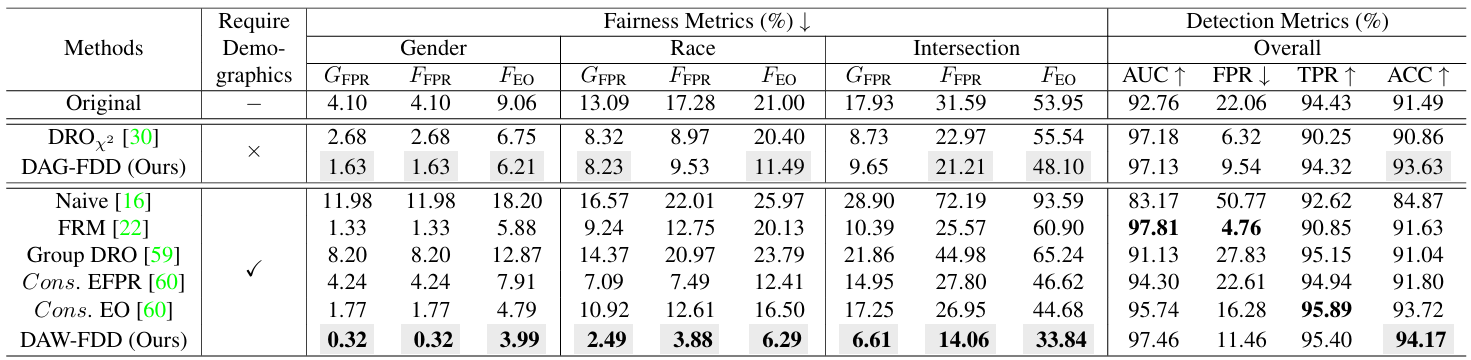
\includegraphics[width=\textwidth]{images/dag_img1.png}
    \caption{Comparison of fairness-aware methods on FF++ using the Xception backbone (adapted from \cite{dag_paper}).}
    \label{fig:ch4_ffpp_xception}
\end{figure}

\begin{figure}[htbp]
    \centering
    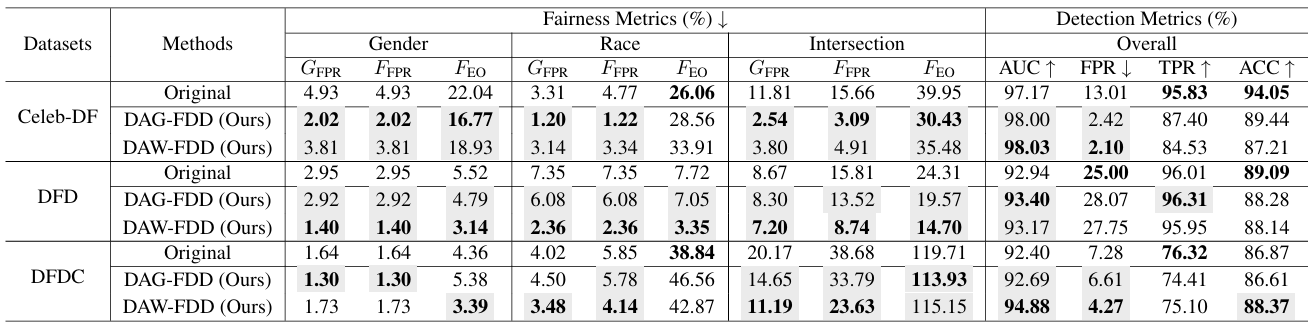
\includegraphics[width=\textwidth]{images/dag_img2.png}
    \caption{Evaluation on Celeb-DF, DFD, and DFDC using Xception (adapted from \cite{dag_paper}). Results show fairness and detection metrics across datasets.}
    \label{fig:ch4_dataset_comparison}
\end{figure}

From Figure~\ref{fig:ch4_ffpp_xception}, the following patterns can be observed:

\begin{itemize}
    \item \textbf{Strong reduction in fairness gaps:}  
    Both DAG-FDD and DAW-FDD significantly lower GFPR/FFPR compared to the original model.

    \item \textbf{DAW-FDD achieves best fairness:}  
    When demographic labels are available, DAW-FDD consistently produces the lowest group disparities.

    \item \textbf{Competitive detection performance:}  
    Improvements in fairness do not come at the cost of AUC or accuracy.

    \item \textbf{Comparison with prior fairness methods:}  
    The proposed methods outperform baselines such as DRO, Group DRO, and constraint-based approaches.
\end{itemize}

\noindent
This confirms that CVaR-based optimisation is effective even in standard in-domain training.

% ------------------------------------------------------------------
\subsection{Cross-Dataset Generalisation}
\label{subsec:ch4_crossdomain}
% ------------------------------------------------------------------

Figure~\ref{fig:ch4_dataset_comparison} evaluates generalisation across datasets.

\begin{itemize}
    \item \textbf{Fairness improvements persist across datasets:}  
    Both DAG-FDD and DAW-FDD continue to reduce disparity outside the training dataset.

    \item \textbf{Robustness to distribution shift:}  
    The method remains effective even when data characteristics change (e.g., DFDC vs FF++).

    \item \textbf{DAW-FDD benefits from group labels:}  
    When demographic structure is available, improvements are more pronounced.

    \item \textbf{DAG-FDD remains practical:}  
    Even without labels, DAG-FDD provides meaningful robustness gains.
\end{itemize}

\noindent
This indicates that the CVaR objective is not overfitting to a specific dataset distribution.

\begin{figure}[htbp]
    \centering
    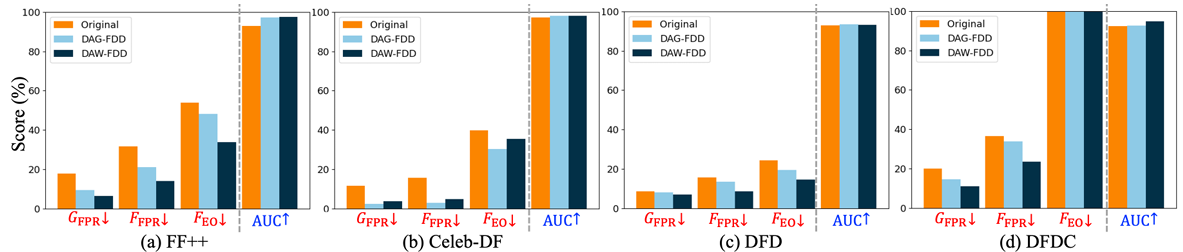
\includegraphics[width=\textwidth]{images/dag_img4.png}
    \caption{Intersectional fairness comparison of the Xception detector across four datasets: FF++, Celeb-DF, DFD, and DFDC (adapted from Figure~1 in \cite{dag_paper}).}
    \label{fig:ch4_intersection_multidataset}
\end{figure}

\begin{figure}[htbp]
    \centering
    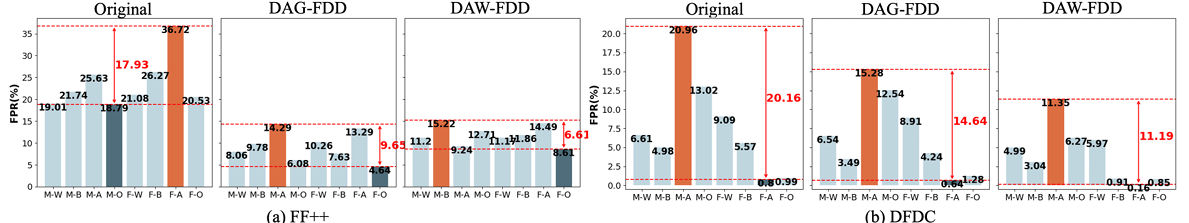
\includegraphics[width=\textwidth]{images/dag_img5.png}
    \caption{FPR comparison of the Xception detector on intersectional groups for FF++ and DFDC (adapted from Figure~2 in \cite{dag_paper}). Orange and dark cyan bars denote the groups with the highest and lowest FPR, respectively, and the red bracket shows the gap, where a smaller value is better.}
    \label{fig:ch4_intersection_fpr_gap}
\end{figure}

Figure~\ref{fig:ch4_intersection_multidataset} provides a more detailed view of the intersectional setting across datasets. It shows that the proposed methods consistently \emph{reduce the fairness gaps for intersection groups while maintaining competitive AUC}. The improvement is visible not only on FF++, but also on Celeb-DF, DFD, and DFDC, which supports the paper's claim that the CVaR-based objectives generalize well beyond a single benchmark.

Figure~\ref{fig:ch4_intersection_fpr_gap} focuses specifically on false-positive disparity across intersection groups. This is especially important because the paper emphasizes FPR as the most practically harmful error mode in deepfake detection. Both DAG-FDD and DAW-FDD reduce the gap between the highest and lowest FPR groups, showing that the fairness objective improves not just average behavior but also worst-group outcomes.

% ------------------------------------------------------------------
\subsection{Backbone Robustness}
\label{subsec:ch4_stability}
% ------------------------------------------------------------------

\begin{figure}[htbp]
    \centering
    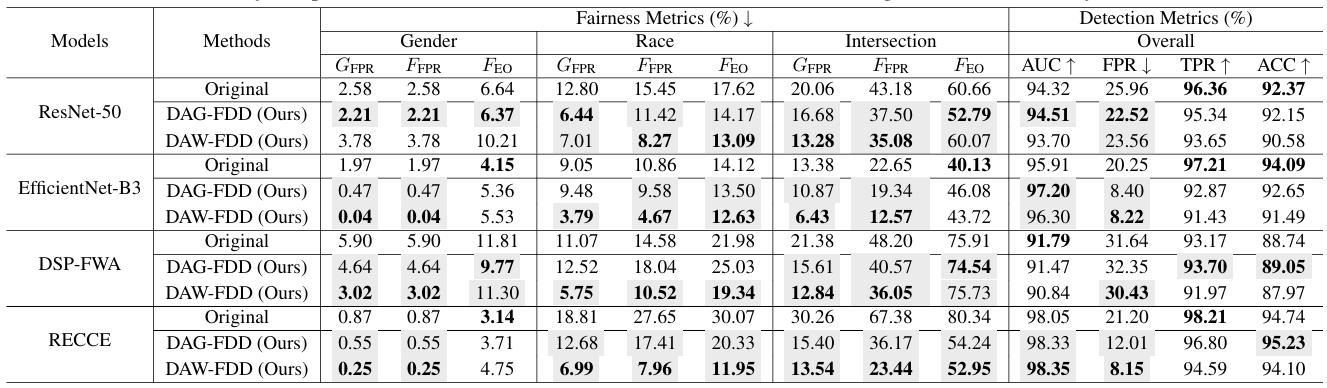
\includegraphics[width=\textwidth]{images/dag_img3.png}
    \caption{Performance across multiple backbones (ResNet-50, EfficientNet-B3, DSP-FWA, RECCE) on FF++ (adapted from \cite{dag_paper}).}
    \label{fig:ch4_backbone_comparison}
\end{figure}

Figure~\ref{fig:ch4_backbone_comparison} demonstrates that the proposed method is not tied to a specific architecture.

\begin{itemize}
    \item \textbf{Backbone-agnostic behaviour:}  
    Fairness improvements are consistent across all evaluated detectors.

    \item \textbf{Stable detection metrics:}  
    Performance remains competitive regardless of architecture.

    \item \textbf{Plug-and-play nature:}  
    The method only modifies the loss function and can be integrated into existing models.
\end{itemize}

% ------------------------------------------------------------------
\subsection{Computational Considerations}
\label{subsec:ch4_efficiency}
% ------------------------------------------------------------------

\begin{itemize}
    \item \textbf{Additional overhead:}  
    Comes from optimisation of CVaR thresholds ($\lambda$, $\lambda_g$).

    \item \textbf{Implementation cost:}  
    Requires binary search or iterative updates.

    \item \textbf{Practical trade-off:}  
    The overhead is modest relative to the fairness gains achieved.
\end{itemize}
 
% ------------------------------------------------------------------

\section{Key Insights for Our Project}
\label{sec:ch4_insights}
% ------------------------------------------------------------------

This paper is useful for our project because it offers a clean way to promote fairness without redesigning the full architecture. The main lesson we draw from it is that \textbf{fairness can be controlled at the optimisation level}. The most important takeaways are as follows.

\begin{enumerate}
    \item Worst-case focus is more informative than average loss when the goal is fair and robust performance.
    \item Hierarchical CVaR is a natural way to handle fairness when both sample-level hardness and group-level imbalance are present.
    \item DAG-FDD is the appropriate formulation when demographic labels are not available.
    \item DAW-FDD is the more structured and more explicit formulation when demographic labels are available.
    \item The top-$k$ or CVaR estimator inside each group is important for handling imbalance between real and fake samples within a demographic group.
\end{enumerate}

% ------------------------------------------------------------------
\section{Conclusion}
\label{sec:ch4_conclusion}
% ------------------------------------------------------------------

In this chapter, we described the CVaR-based fairness framework for deepfake detection and explained how it leads to two related methods: DAG-FDD and DAW-FDD. DAG-FDD handles the setting where demographic labels are absent and works through latent worst-case sample optimisation. DAW-FDD extends the same idea to the demographic-aware setting by adding group-level CVaR and per-group top-$k$ estimation.

The main contribution of the paper is that it replaces average-risk training with a more robust and fairness-sensitive objective, allowing the detector to pay greater attention to the hardest samples and the worst-performing groups, which in turn improves fairness without significantly compromising detection quality. For our own work, this paper serves as a strong reference for using robust optimisation as a fairness mechanism in deepfake detection.
 %cvar_deepfake
%% ============================================================
%%  CHAPTER 5 — Proposed Solution: FAIR-FRFT Architecture
%%  Ethics in AI: Emphasis on Fairness
%%  CSC-391 Technical Communication, IIT Roorkee
%% ============================================================
 
\chapter{Targeting a Critical Gap in Deepfake Detectors}
\label{ch:proposed}
 
\vspace{0.5em}
\noindent\rule{\textwidth}{0.4pt}
\textbf{Declaration of Contributions:} This chapter was developed by
\textit{Siddharth Gupta} and \textit{Aryan Choudhary}, the former contributed to the conceptualisation and theoretical design of the autoencoder architecture and the debiasing framework, based on an extensive review of existing literature, while the later contributed to the theoretical formulation and design of the CVaR-based fairness module.
\noindent\rule{\textwidth}{0.4pt}
\vspace{1em}

\bigskip


 
This chapter presents \textbf{FAIR-FRFT} (\emph{Fairness-Aware
Fractional Fourier Transform for Deepfake Detection}), our proposed
framework for demographically fair deepfake detection.  Unlike prior
methods that append fairness as a post-hoc constraint on top of an
existing architecture, FAIR-FRFT treats fairness as a
\emph{fundamental design principle}, embedding demographic invariance
directly into the representation-learning process through three
tightly coupled components: (i) a hybrid spatial--frequency encoder
driven by the Fractional Fourier Transform, (ii) an adversarial
autoencoder with a Gradient Reversal Layer, and (iii) a
CVaR-based tail-risk fairness objective.  Together, these components
ensure that the learned latent representations are simultaneously
deepfake-discriminative and demographic-agnostic.

% ------------------------------------------------------------------
\section{Problem Statement}
\label{sec:problem_statement}
% ------------------------------------------------------------------

Deepfake detectors are not necessarily fair across demographic groups.
A model may achieve strong overall accuracy while still producing
systematically different error rates for different communities. This occurs when the detector learns correlations present in the training data that do not generalise fairly across groups.

In the context of deepfake detection, such bias is especially problematic because the impact of an error can be severe. A detector that performs well on one community but poorly on another may create uneven trust and unequal risk. 

\subsubsection{Illustrative Scenario}
\label{subsec:problem_example}

Consider an election setting in which a deepfake speech is circulated
publicly against a political candidate. Suppose the detector, due to its inherent bias and limitations in learned representations, incorrectly labels the speech as genuine rather than synthetic. Such a failure may allow the manipulated content to spread widely, potentially triggering public unrest, misleading voters and damaging the candidate's reputation. This example highlights why fairness in deepfake detection is not merely a technical concern, but a \emph{matter of real-world safety and social responsibility}.
 
% ------------------------------------------------------------------
\section{Overview of the FAIR-FRFT Architecture}
\label{sec:architecture_overview}
% ------------------------------------------------------------------
 
Figure~\ref{fig:fairfrft_architecture} provides a complete view of the
FAIR-FRFT pipeline.  At the highest level, the framework comprises
four functional blocks:
 
\begin{enumerate}
  \item \textbf{FrFT pre-processor}  The input image $\mathbf{x}$
        is mapped to the hybrid spatial frequency domain via the
        Fractional Fourier Transform, yielding frequency maps
        $\mathbf{x}' = \mathcal{F}_\alpha^{(d)}(\mathbf{x})$.
  \item \textbf{Adversarial autoencoder}  An encoder
        $E_\theta$ compresses $\mathbf{x}'$ into a latent
        representation $\mathbf{z}$; a decoder $G_\theta$
        reconstructs the spatial-domain image $\hat{\mathbf{x}}$
        from $\mathbf{z}$.  The cycle is closed by re-encoding the
        reconstruction for latent consistency.
  \item \textbf{Demographic adversary}  A demographic classifier
        $D_\phi$ attempts to predict the protected group $g$ from
        $\mathbf{z}$.  Gradient reversal forces the encoder to
        \emph{maximise} the adversary's error, thereby stripping
        demographic information from the latent space.
  \item \textbf{Binary Real/Fake classifier}  After the encoder has
        converged to a fair representation, a lightweight
        classifier $C_\psi$ is trained on the frozen $\mathbf{z}$
        to detect real versus fake faces.
\end{enumerate}
 
% ------------------------------------------------------------------
\section{Fractional Fourier Transform Pre-processing}
\label{sec:frft_preproc}
% ------------------------------------------------------------------
 
The Fractional Fourier Transform (FrFT), introduced in
Section~\ref{sec:frft}, serves as the input representation for
FAIR-FRFT.  For an order parameter $\alpha \in [0,1]$, the
2-D FrFT of an image $\mathbf{x}$ is computed channel-wise as:
\begin{equation}
  \mathbf{x}' = \mathcal{F}_\alpha^{(d)}(\mathbf{x})
  \label{eq:frft_preproc}
\end{equation}

\begin{equation}
  \mathcal{F}_\alpha[f](u)
  = e^{-i\pi u^2 \cot\alpha}
    \cdot \mathrm{FFT}\!\left[f(t)\,e^{-i\pi t^2 \cot\alpha}\right]\!(u\csc\alpha)
\end{equation}

\begin{figure}[h]
    \centering
    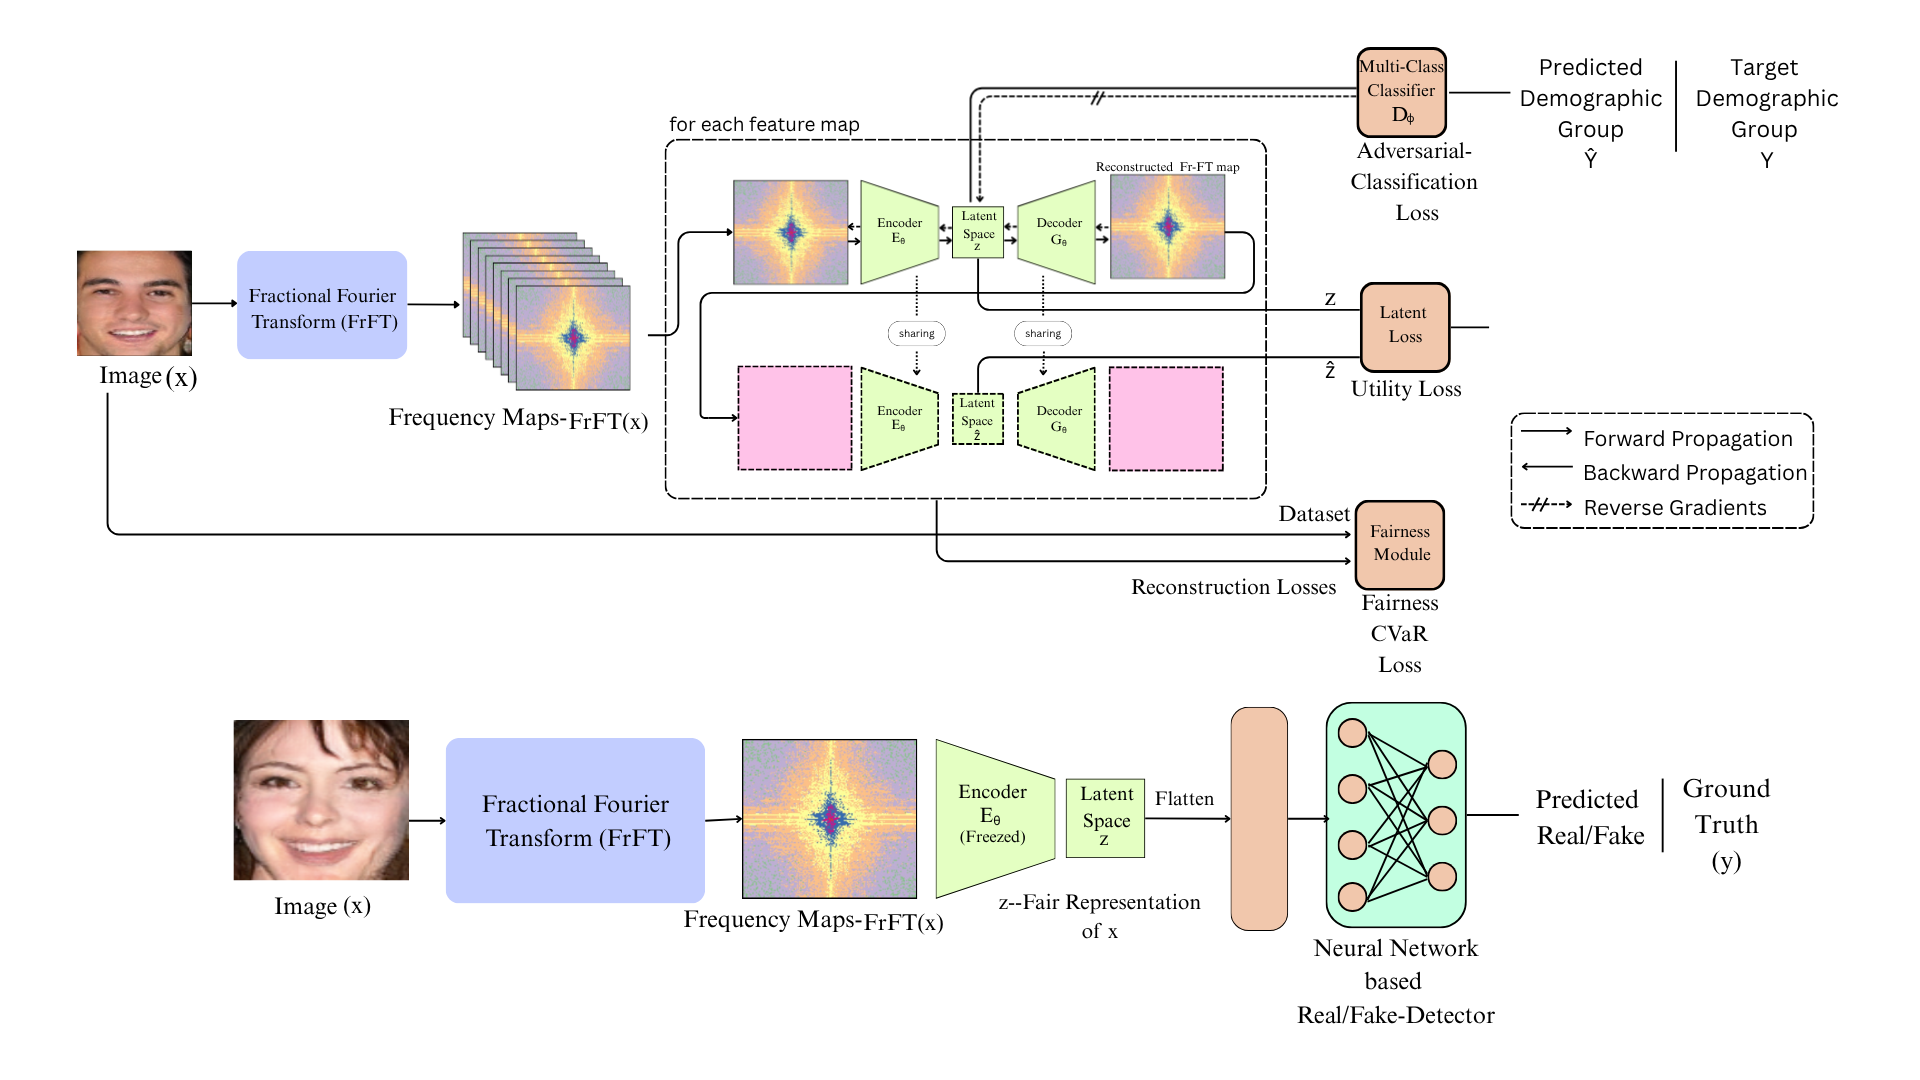
\includegraphics[width=1\textwidth]{images/FAIRFRFT.png}
    \caption{FAIR-FRFT Architecture. Top: FrFT-transformed input $x'$ is encoded by $E_{\theta}$ into latent $z$, reconstructed by $G_{\theta}$ to $\hat{x}$, and re-encoded for consistency. The model includes demographic adversary $D_{\phi}$, real/fake head $R_{\psi}$, and CVaR fairness loss. Bottom: After training, the encoder is frozen and a classifier predicts real/fake labels from the learned fair representation.}
    \label{fig:fairfrft_architecture}
\end{figure}

 
% ------------------------------------------------------------------
\section{Adversarial Autoencoder}
\label{sec:adv_ae}
% ------------------------------------------------------------------
 
\subsubsection{Encoder and Decoder}
\label{subsec:enc_dec}
 
The encoder $E_\theta : \mathbb{R}^{H \times W \times C}
\to \mathbb{R}^d$ maps the FrFT-transformed image to a
$d$-dimensional latent vector:
\begin{equation}
  \mathbf{z} = E_\theta(\mathbf{x}').
  \label{eq:encoder}
\end{equation}
We implement $E_\theta$ as a three-layer CNN with filter counts 32, 64 and 128. Layer Normalization after each convolution and additive Gaussian noise ($\sigma = 0.05$) for regularisation. Critically, no non-linear activation function is applied after the final layer; this preserves the sign of latent activations, which carries phase information propagated from the FrFT.
 
The decoder $G_\theta : \mathbb{R}^d \to
\mathbb{R}^{H \times W \times C}$ reconstructs the spatial-domain
image:
\begin{equation}
  \hat{\mathbf{x}} = G_\theta(\mathbf{z}).
  \label{eq:decoder}
\end{equation}
$G_\theta$ is a symmetric CNN with transposed convolutions and skip connections from the corresponding encoder layers, mirroring the U-Net paradigm to recover fine spatial detail. The reconstructed image is then re-processed through FrFT and re-encoded:
\begin{equation}
  \hat{\mathbf{x}}' = \mathcal{F}_\alpha^{(d)}(\hat{\mathbf{x}}),
  \qquad
  \hat{\mathbf{z}} = E_\theta(\hat{\mathbf{x}}')
  \label{eq:cycle}
\end{equation}
 
\subsubsection{Latent Consistency Objective}
\label{subsec:lat_consistency}
 
Rather than enforcing pixel-level reconstruction which would force the model to attend to demographic appearance details we enforce \emph{latent-space consistency}. The latent consistency loss comprises an $\ell_2$ term and a cosine-similarity term:
\begin{equation}
  \mathcal{L}_{\mathrm{lat}}
  \;=\;
  \bigl\|\hat{\mathbf{z}} - \mathrm{sg}(\mathbf{z})\bigr\|_2^2
  \;+\;
  \beta\,\bigl(1 - \cos(\hat{\mathbf{z}},\,\mathrm{sg}(\mathbf{z}))\bigr),
  \quad \beta = 1.0
  \label{eq:lat_loss}
\end{equation}
where $\mathrm{sg}(\cdot)$ denotes the \emph{stop-gradient} operator (the target $\mathbf{z}$ is treated as a constant during the backward pass). By constraining the encoder to produce latents that survive a decode re-encode cycle, we encourage the representation to capture \emph{semantic deepfake cues} (which persist through reconstruction) while discarding superficial appearance variations such as skin tone and facial structure (which are smoothed away by the decoder).
 
% ------------------------------------------------------------------
\section{Adversarial Demographic Debiasing via Gradient Reversal}
\label{sec:adv_debias}
% ------------------------------------------------------------------
 
\subsubsection{Demographic Classifier}
\label{subsec:dem_clf}
 
A demographic classifier $D_\phi : \mathbb{R}^d \to \mathbb{R}^{|\mathcal{G}|}$ maps the latent representation to a probability distribution over demographic groups.  It is implemented as a two-layer MLP with Layer Normalisation and Max-Norm constraints ($c_{\max} = 3.0$) to bound its complexity.  The adversarial classification loss is:
\begin{equation}
  \mathcal{L}_{\mathrm{adv\text{-}clf}}
  \;=\;
  \mathbb{E}_{\mathbf{x},g}\!\bigl[
    \mathrm{CE}\!\bigl(D_\phi(\mathrm{GRL}(\mathbf{z})),\, g\bigr)
  \bigr],
  \label{eq:adv_clf}
\end{equation}
where $\mathrm{GRL}(\cdot)$ is the Gradient Reversal Layer defined in Eq.~\ref{eq:grl}.
 
\subsubsection{Minimax Training Objective}
\label{subsec:minimax}
 
The encoder and demographic classifier engage in a minimax game:
\begin{equation}
  \min_{\theta}\;\max_{\phi}\;
  \mathcal{L}_{\mathrm{AE}}
  \;=\;
  \lambda_{\mathrm{lat}}\,\mathcal{L}_{\mathrm{lat}}(\theta)
  \;+\;
  \lambda_{\mathrm{fair}}\,\mathcal{L}_{\mathrm{fair}}(\theta)
  \;-\;
  \lambda_{\mathrm{adv}}\,\mathcal{L}_{\mathrm{adv\text{-}clf}}(\theta,\phi).
  \label{eq:minimax}
\end{equation}
The negative sign on $\mathcal{L}_{\mathrm{adv\text{-}clf}}$ causes the encoder to \emph{maximise} the adversary's classification error equivalently, to remove demographic information from $\mathbf{z}$.  The GRL makes this implicit: during the forward pass it acts as the identity; during back-propagation it negates the gradient by the reversal strength $\lambda_{\mathrm{grl}}$ (Eq.~\ref{eq:grl}),  avoiding the need for alternating optimisation.

 
% ------------------------------------------------------------------
\section{CVaR Fairness Loss}
\label{sec:cvar_fair}
% ------------------------------------------------------------------
 
Adversarial debiasing removes demographic information from $\mathbf{z}$ in an \emph{average} sense, but may still leave vulnerable subgroups under-served.  To protect these subgroups, we propose to augment the training objective with a \emph{group-level CVaR} fairness loss (see Section~\ref{sec:cvar}):
\begin{equation}
  \mathcal{L}_{\mathrm{fair}}
  \;=\;
  \max_{y,\,a}\;
  \mathrm{CVaR}_\alpha\!\bigl(\ell(\mathbf{x}, y) \mid y, a\bigr),
  \label{eq:fair_loss}
\end{equation}
where $y \in \{0,1\}$ is the real/fake label, $a$ is the demographic group, and the inner CVaR is taken over the loss distribution of that demographic--label cell.  Taking the $\max$ over all $(y, a)$ combinations focuses optimisation on the \emph{worst-performing subgroup}, ensuring Equalized Odds across the population.  This connects directly to the group-level CVaR formulation of Eq.~\ref{eq:group_cvar}.
 
% ------------------------------------------------------------------
\section{Model Pipeline}
\label{sec:training_strategy}
% ------------------------------------------------------------------
 
The proposed model pipeline ought to be trained in two stages:
 
\subsubsection{Stage 1 : Fair Representation Learning}
\label{subsec:stage1}
The adversarial autoencoder is to be trained end-to-end to learn demographic-agnostic semantically meaningful representations:
\begin{equation}
  \theta^{(1)},\,\phi^*
  \;=\;
  \operatorname*{arg\,min}_{\theta}\;
  \operatorname*{arg\,max}_{\phi}\;
  \mathcal{L}_{\mathrm{AE}}(\theta, \phi).
  \label{eq:stage1}
\end{equation}

\subsubsection{Stage 2 : Binary Classification}
\label{subsec:stage2}
 
Once the encoder has converged, $E_\theta$ is \emph{frozen} and a separate real/fake classifier $C_\psi$ ought to be trained on the fixed representations:
\begin{equation}
  \psi^*
  \;=\;
  \operatorname*{arg\,min}_{\psi}\;
  \mathcal{L}_{\mathrm{clf}}(\psi;\,\theta^{(1)})
  \;=\;
  \mathbb{E}_{\mathbf{x},y}\!\bigl[
    \mathrm{CE}\!\bigl(C_\psi(\mathbf{z}),\,y\bigr)
  \bigr].
  \label{eq:stage2}
\end{equation}
Decoupling representation learning from classification prevents the
classifier's cross-entropy gradient from re-introducing demographic
bias into $\mathbf{z}$.
 
 
% ------------------------------------------------------------------
\section{Chapter Summary}
\label{sec:ch5_summary}
% ------------------------------------------------------------------
 
This chapter presented FAIR-FRFT, our proposed fairness-aware
deepfake detection framework.  The key design decisions and their
justifications are:
 
\begin{itemize}
  \item \textbf{FrFT pre-processing} maps images into a hybrid spatial frequency domain where deepfake artefacts are more discriminative and less entangled with demographic
        appearance features.
  \item \textbf{Latent consistency training} replaces pixel reconstruction with a semantic cycle-consistency objective, preventing the autoencoder from memorising demographic appearance cues.
  \item \textbf{Gradient Reversal} implements adversarial debiasing within a single forward--backward pass, actively removing demographic information from the latent space without alternating optimisation. 
  \item \textbf{CVaR fairness loss} complements adversarial 
        debiasing by directly penalising worst-case subgroup  performance, linking the training objective to the Equalized Odds fairness criterion.
  \item \textbf{Two-stage training} decouples fair
        representation learning from task-specific
        classification, preventing the classifier's gradient
        from re-introducing bias.
\end{itemize} %proposed architecture
% ============================================================
\chapter{Conclusion, Future Work, and Industry Approaches}
% ============================================================
\label{ch:conclusion}


\vspace{0.5em}
\noindent\rule{\textwidth}{0.4pt}
\noindent\textbf{Declaration of Contributions:}
This chapter was compiled and authored by \textit{Vishesh Gupta}, who
interpreted the fairness metrics, analysed experimental results, and connected
the technical findings with real-world AI systems deployed by industry leaders.
\textit{Nitin Agiwal} contributed the concluding synthesis of bias and fairness
across the machine-learning pipeline. All team members cross-checked factual claims and references for accuracy.
\noindent\rule{\textwidth}{0.4pt}
\vspace{1em}

\bigskip

This chapter consolidates the key findings of the report, outlines directions
for future investigation, and situates the research within the broader landscape
of how major AI organisations currently address algorithmic fairness.
We begin with a synthesis of our conclusions, followed by concrete open
problems, and close with a comparative survey of fairness approaches adopted by
OpenAI, Google, and IBM.

% ============================================================
\section{Conclusion}
% ============================================================

Bias in AI is a systemic problem deeply embedded across the entire
machine-learning pipeline, from data collection and model training through to
evaluation.
It arises due to historical inequalities reflected in data, underrepresentation
of certain demographic groups, and human subjectivity in labelling and feature
selection~\cite{propublica_compas}.
Real-world case studies such as the COMPAS recidivism algorithm and Amazon's
hiring system demonstrate that such biases can directly harm marginalised
communities and perpetuate existing social inequalities at scale.

Traditional evaluation metrics such as accuracy are insufficient for assessing
fairness: models can achieve high overall performance while producing
disproportionately harmful outcomes for specific demographic groups.
This work examined the FD-VAE architecture~\cite{park2020readme} as a
principled approach to fair representation learning.
FD-VAE addresses the fundamental flaw in prior methods, most notably
FFVAE, by introducing a three-way disentanglement of the latent space into
\emph{target} ($z_t$), \emph{protected} ($z_p$), and \emph{mutual} ($z_m$)
attribute components, ensuring that the shared predictive information is
exploited without leaking demographic signals into downstream classifiers.

The incorporation of Conditional Value-at-Risk (CVaR) loss~\cite{ju2024fairness}
further strengthens robustness by focusing training on worst-performing
subgroups rather than on average-case behaviour, encouraging fairness even in
the absence of explicit group labels.
The proposed pipeline extends these ideas to deepfake detection by combining
Fractional Fourier Transform (FrFT) preprocessing~\cite{ozaktas2001frft},
latent consistency enforcement, adversarial debiasing, and CVaR fairness loss.
Together, these components aim to build a detection system that is not only
accurate but equitable across demographic groups.

The ultimate goal is to develop AI systems that are \textbf{trustworthy},
\textbf{socially responsible}, and \textbf{fair by design} rather than as an
afterthought.

% ============================================================
\section{Future Work}
% ============================================================

Several directions remain open for further investigation.

\paragraph{Empirical Validation.}
The proposed FrFT-based pipeline has been designed at an architectural level;
empirical validation on standard benchmarks such as CelebA and UTK Face
datasets is needed to quantitatively confirm its fairness--accuracy trade-offs
against existing baselines including FFVAE and FD-VAE~\cite{park2020readme}.

\paragraph{Multi-Attribute Fairness.}
The current approach assumes binary protected attributes such as gender.
Extending the framework to handle multiple intersecting sensitive attributes
simultaneously, race, age, and gender combined, presents a non-trivial
challenge that warrants dedicated study.
Intersectional fairness metrics that jointly penalise subgroup disparities
would be a natural first step.

\paragraph{CVaR Hyperparameter Scheduling.}
The CVaR parameter $\alpha$ critically governs the fairness--accuracy
trade-off~\cite{ju2024fairness}.
A systematic sensitivity analysis and an adaptive scheduling strategy for
$\alpha$ during training could improve generalisation across datasets with
varying demographic distributions.

\paragraph{Training Stability of Adversarial Objectives.}
While adversarial debiasing is effective, it introduces the training
instability common to minimax objectives.
Exploring alternative decorrelation strategies, such as kernel-based
independence tests or information-theoretic regularisation, may yield more
stable and scalable training dynamics.

\paragraph{Broader Application Domains.}
The applicability of this pipeline to high-stakes domains beyond deepfake
detection, including medical imaging, credit scoring, and hiring
systems, represents a promising and socially impactful direction.
Each domain introduces unique distributional challenges (e.g.\ class imbalance
in medical data, legally protected attributes in credit scoring) that would
require careful adaptation of the proposed fairness constraints.

% ============================================================
\section{How AI Industry Leaders Address Fairness}
% ============================================================

Beyond academic research, major technology companies have developed their own
fairness frameworks and tools.
These approaches span training-time interventions, post-processing audits, and
open-source toolkits.
Three leading efforts are examined below.

% , , , , , , , , , , , , , , , , , , , , 
\subsection{OpenAI ,  Reinforcement Learning with Human Feedback (RLHF)}
% , , , , , , , , , , , , , , , , , , , , 

OpenAI employs Reinforcement Learning with Human Feedback
(RLHF)~\cite{ouyang2022rlhf} to align model behaviour with human values,
including fairness.
The key techniques include:

\begin{itemize}[leftmargin=2em]
    \item \textbf{Human reviewers} who guide the model toward safe, unbiased
          responses through preference-based feedback.
    \item \textbf{Bias evaluation benchmarks} that test model outputs across
          demographic groups before deployment.
    \item \textbf{Content moderation layers} that filter outputs in real time
          to prevent discriminatory or toxic content.
\end{itemize}

The primary goal of RLHF in this context is to ensure that language models
avoid generating discriminatory responses or perpetuating harmful stereotypes.
Human oversight is central to this approach, making it effective but also
resource-intensive and dependent on the diversity of human reviewers.

% , , , , , , , , , , , , , , , , , , , , 
\subsection{Google ,  Responsible AI Policies}
% , , , , , , , , , , , , , , , , , , , , 

Google has embedded fairness considerations into its model development
lifecycle through its Responsible AI framework, applied prominently in the
Gemini family of models~\cite{gemini2023}.
The key techniques are:

\begin{itemize}[leftmargin=2em]
    \item \textbf{Safety tuning during training}, where dataset composition and
          sampling strategies are adjusted to reduce demographic disparities
          before training begins.
    \item \textbf{Dataset filtering} to remove or rebalance data that may
          encode historical inequalities.
    \item \textbf{Fairness checks} that explicitly test for gender-, race-, and
          culture-based disparities in model outputs.
\end{itemize}

Google's approach addresses bias at the source, during data preparation and
model training, and is generally more effective than post-hoc correction.
However, ensuring comprehensive coverage across all demographic dimensions
remains an ongoing challenge.

% , , , , , , , , , , , , , , , , , , , , 
\subsection{IBM ,  AI Fairness 360 (AIF360)}
% , , , , , , , , , , , , , , , , , , , , 

IBM has released AI Fairness 360 (AIF360)~\cite{aif360}, an open-source Python
toolkit designed to help practitioners detect and mitigate bias across the full
machine-learning pipeline.
The toolkit provides:

\begin{itemize}[leftmargin=2em]
    \item \textbf{Bias detection algorithms} that quantify disparate impact,
          statistical parity, and other fairness metrics.
    \item \textbf{Bias mitigation algorithms} categorised by intervention stage:
    \begin{itemize}[leftmargin=1.5em]
        \item \textit{Pre-processing:} Reweighting and disparate impact remover
              applied to training data to reduce bias at its source, ensuring
              that the model learns from a more balanced representation of the
              data.
        \item \textit{In-processing:} Adversarial debiasing and prejudice
              remover applied during model training, actively guiding the
              learning algorithm to reduce bias while it is being trained.
        \item \textit{Post-processing:} Calibrated equalized odds and reject
              option classification applied to model outputs, adjusting final
              predictions to ensure more equitable outcomes across different
              groups.
    \end{itemize}
\end{itemize}

AIF360's open-source nature makes it widely accessible and adaptable across
industries.
It supports a wide range of fairness metrics and can be integrated into
existing machine-learning workflows with minimal overhead.

% , , , , , , , , , , , , , , , , , , , , 
\subsection{Comparative Summary}
% , , , , , , , , , , , , , , , , , , , , 

Table~\ref{tab:industry_comparison} summarises the three approaches along the
dimensions of primary strategy, key techniques, and the types of harm each is
designed to avoid.

\begin{table}[H]
\centering
\renewcommand{\arraystretch}{1.35}
\begin{tabularx}{\textwidth}{lXXX}
\toprule
\textbf{Company} & \textbf{Approach} & \textbf{Techniques} & \textbf{What It Avoids} \\
\midrule
\textbf{OpenAI} \newline (ChatGPT / GPT-4) &
    RLHF (Reinforcement Learning with Human Feedback)~\cite{ouyang2022rlhf} &
    Human reviewers guide safe responses; bias evaluation benchmarks; content
    moderation layers &
    Toxic outputs; discriminatory responses \\
\addlinespace
\textbf{Google} \newline (Gemini) &
    Responsible AI Policies~\cite{gemini2023} &
    Safety tuning during training; dataset filtering &
    Gender-, race-, and culture-based disparities (via fairness checks) \\
\addlinespace
\textbf{IBM} \newline (AIF360) &
    Open-source Fairness Toolkit~\cite{aif360} &
    Bias detection; bias mitigation algorithms at pre-, in-, and
    post-processing stages &
    Algorithmic bias across protected groups \\
\bottomrule
\end{tabularx}
\caption{Comparison of industry approaches to AI fairness.}
\label{tab:industry_comparison}
\end{table} %conclusion and future work
% ============================================================
%  BIBLIOGRAPHY
% ============================================================
\cleardoublepage
\addcontentsline{toc}{chapter}{Bibliography}
\bibliographystyle{unsrt}       % numeric, unsorted — matches the original
\bibliography{references}       % references.bib file

\end{document}